%!TEX encoding = UTF-8 Unicode
%\part{Real-Time Hybrid Test Method}
\chapter{Hybrid Testing Method}
\label{rthytem}
In this chapter, the hybrid testing method is introduced as a classification according to equipment type. The hybrid testing method is mainly divided into shaking table experiment and UTM experiment by its equipment type. First, the hybrid testing method using the shaking table is split into the substructuring test method which tests the partial structural system separately, and the hybrid shaking table testing method by installing building structure with nonlinear mass typed vibration control devices such as TLD, TLCD, and TLMD. Secondly, in the case of MR damper which is a type of semi-active friction damper, it is very difficult to implement hybrid shaking table testing installed in an actual building. Therefore, the MR damper is installed in a universal testing machine (UTM), and a hybrid testing method is implemented by simulating the MR damper behavior mounted in a real scaled building. This subject will consider with chapter~\ref{chap:rthytem-mrdamper}.

\section{Substructuring technique}
\label{chap:realtimesubstrct}

The most substructuring techniques focus on the nonlinear behavior of the lower stories, which are selected as the experimental substructure. Accordingly, the upper stories are considered as the numerical substructure in those conventional substructuring techniques. Differently, from those researches, these studies address the substructuring technique for the shaking table test of a building structure adopting the upper stories as the experimental substructure and the lower stories as the analytical substructure. Figure~\ref{fig:2-1} shows the conceptual difference between the conventional and the proposed substructuring techniques as part of a hybrid testing method. 
The necessity of testing the upper substructure is found in diverse structures. For example, the wind-induced acceleration response of slender building structures is usually tremendous in the top story, and detailed experiment for this upper part of the building structure may be required, since excessive acceleration response may be harmful to human comfort or high precision equipment. Also, in some cases, a light appendage, for example, a penthouse, a small housing for mechanical equipment and an advertising billboard, may vibrate excessively rather than the primary structure. Besides, to suppress excessive vibration induced by winds and earthquakes, a tuned mass damper or tuned liquid damper is employed on the top story of the high-rise building, and its performance should be verified in the laboratory before installation. Finally, the base isolation system to protect expensive machinery housed in a building structure needs experimental verification for a certain level of earthquake.

\begin{figure}[ht]
\centering

\subfigure[conventional method]{
   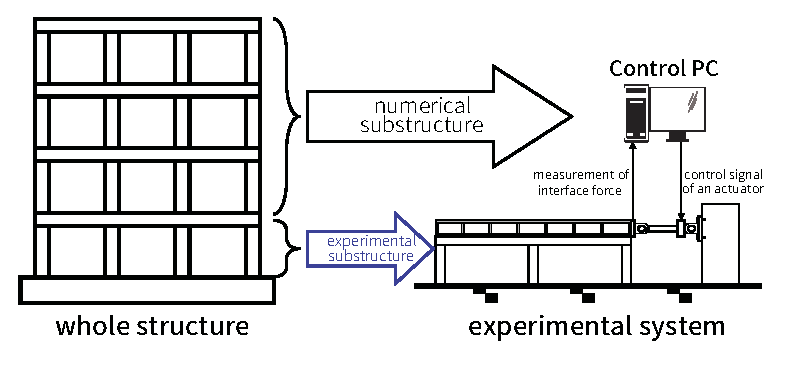
\includegraphics[scale =1] {figure/2_1a.eps}
   \label{fig:2-1a}
 }

 \subfigure[proposed method]{
   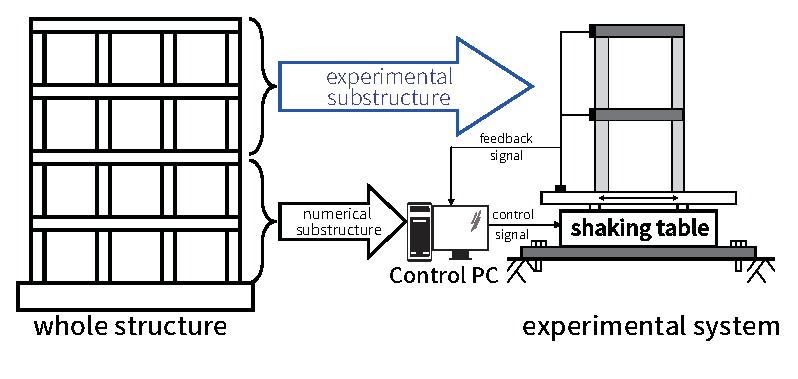
\includegraphics[scale =1] {figure/2_1b.eps}
   \label{fig:2-1b}
 }

\label{fig:2-1}
\caption{Conceptual illustrations of the substructuring methods}
\end{figure}

On these backgrounds, this subsection proposes a shaking table testing method using the upper part of a building structure as the experimental substructure based on the acceleration feedback from the experimental substructure. Also, the proposed method is verified experimentally through real-time implementation. Figure~\ref{fig:2-2} illustrates the schematic diagram of the proposed testing method in this study. At first, the interface force acting between the upper experimental and lower numerical substructures is calculated based on the acceleration feedback of the experimental substructure which is mounted on shaking table. Then the interface acceleration required to replicate the dynamic behavior of the whole structure is calculated from the numerical substructure subjected to the interface force and assumed base motion for the entire structure. Finally, shaking table excites the upper experimental substructure according to the command signal from the shaking table controller. The series of above processes are performed during a single time interval and repeated over the entire duration of the experiment.

\begin{figure}[ht]
\centering
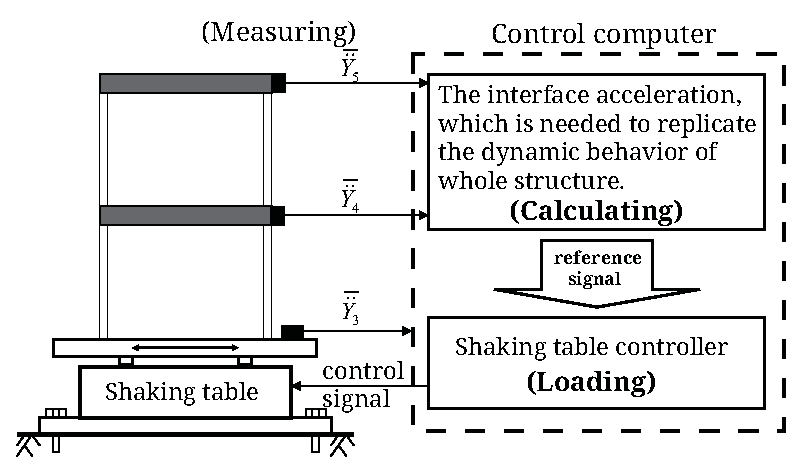
\includegraphics[scale =1] {figure/2-2.eps}
\label{fig:2-2}
\caption{Schematic diagram of the proposed method}
\end{figure}

\subsection{Formulation and Implementation Methodology}
\subsubsection{Experimental and Numerical Substructures}\label{2-2-1}
This subsection addresses physical interpretation and formulation of splitting the whole structure into the experimental and numerical substructures. A two-step process is carried out to formulate the equations of motion for those two substructures; separating the experimental substructure from the whole structure and constructing experimental substructure mounted on the shaking table and numerical substructures with external loads on the cutting plane, as shown in Figure~\ref{fig:2-3}. 

The equation of motion of the whole shear-type building structure subjected to the ground acceleration, $\ddot{Y}_g (t)$, is represented in Figure~\ref{fig:2-3a} and expressed as

\begin{equation}\label{eq:2-1}
\matr{M}\matr{\ddot{Y}}(t)+\matr{C}\matr{\dot{Y}}(t)+\matr{K}\matr{Y}(t) = \matr{p}(t)
\end{equation}

where, $\matr{Y}(t)$ is the $n \times 1$ vector of the absolute floor displacements given by $\left\{Y_{1},Y_{2},...,Y_{n}\right\}^{\top}$, and $\matr{p}(t)$ is the $n \times 1$ vector of the external force given by $\left\{0,...,0,c_{1}\dot{Y}_{g}(t)+k_{1}Y_{g}(t)\right\}^{\top}$, $\matr{M}$, $\matr{C}$ and $\matr{K}$ are the structural mass, damping and stiffness matrices, respectively, and expressed as follows.

\begin{equation}\label{eq:2-2}
\begin{aligned}
\matr{M} = \begin{bsmallmatrix} m_{n}&&&&&&\\&m_{n-1}&&&&&\\&&\ddots&&&&\\ \hline&&&m_{m}&&&\\&&&&m_{m-1}&&\\&&&&&\ddots&\\&&&&&&m_{1} \end{bsmallmatrix},\\
\matr{C} = \begin{bsmallmatrix} c_{n}&-c_{n}&&&&&\\-c_{n}&c_{n}+c_{n-1}&-c_{n-1}&&&&\\&\ddots&\ddots&\ddots&&&\\\hline&&-c_{m+1}&c_{m+1}+c_{m}&-c_{m}&&\\&&&-c_{m}&c_{m}+c_{m-1}&-c_{m-1}&\\&&&&\ddots&\ddots&\ddots&\\&&&&&-c_{2}&c_{2}+c_{1} \end{bsmallmatrix},\\
\matr{K} = \begin{bsmallmatrix} k_{n}&-k_{n}&&&&&\\-k_{n}&k_{n}+k_{n-1}&-k_{n-1}&&&&\\&\ddots&\ddots&\ddots&&&\\\hline&&-k_{m+1}&k_{m+1}+k_{m}&-k_{m}&&\\&&&-k_{m}&k_{m}+k_{m-1}&-k_{m-1}&\\&&&&\ddots&\ddots&\ddots&\\&&&&&-k_{2}&k_{2}+k_{1} \end{bsmallmatrix}
\end{aligned}
\end{equation}

The experimental and numerical substructures are separated from the whole structure by cutting at their interface, as shown in Figure~\ref{fig:2-3b}. Mathematically, this operation means separating the equations included in Eq.~\eqref{eq:2-1} into two groups of which one corresponds to the upper part DOF, and the other corresponds to the lower part DOF. The dotted line in Eq.~\eqref{eq:2-2} divides those two groups, and the resulting two equations of motions are written as

\begin{equation}\label{eq:2-3}
\matr{M}_{E}\matr{\ddot{Y}}_{E}(t)+\matr{C}_{E}(t)\matr{\dot{Y}}_{E}(t)+\matr{K}_{E}\matr{Y}_{E}(t) = \matr{p}_{E}(t)
\end{equation}

\begin{equation}\label{eq:2-4}
\matr{M}_{N}\matr{\ddot{Y}}_{N}(t)+\matr{C}_{N}(t)\matr{\dot{Y}}_{N}(t)+\matr{K}_{N}\matr{Y}_{N}(t) = \matr{p}_{N}(t)
\end{equation}

where, subscripts $E$ and $N$ denote the experimental and numerical substructures, respectively. $\matr{Y}_{E}$ and $\matr{Y}_{N}$ are an $l \times 1$ vector given by $\left\{Y_{E(1)},Y_{E(2)},\right.$ $\left....,Y_{E(l)}\right\}^{\top}$ and an $m \times 1$ vector given by $\left\{Y_{N(1)},Y_{N(2)},...,Y_{N(m)}\right\}^{\top}$, respectively. Accordingly, $n$, the length of the displacement vector, shown in Eq.~\eqref{eq:2-1} equals to $m+l$. Also, $Y_{E(1)}$, $Y_{E(l)}$, $Y_{N(1)}$ and $Y_{N(m)}$ in Eq.'s \eqref{eq:2-3} and \eqref{eq:2-4} correspond to $Y_{m+1}$, $Y_{n}$, $Y_{1}$ and $Y_{m}$ in Eq.~\eqref{eq:2-1}, respectively. The mass, damping and stiffness matrices and the external force vectors in Eq.~\eqref{eq:2-3} and \eqref{eq:2-4} are expressed as follows.

\begin{equation}\label{eq:2-5}
\begin{aligned}
\matr{M}_{E} = \begin{bsmallmatrix} m_{E(l)}&&&&\\&m_{E(l-1)}&&&\\&&\ddots&&\\&&&m_{E(2)}&\\&&&&m_{E(1)} \end{bsmallmatrix},\\
\matr{C}_{E} = \begin{bsmallmatrix} c_{E(l)}&-c_{E(l)}&&&&\\-c_{E(l)}&c_{E(l)}+c_{E(l-1)}&-c_{E(l-1)}&&\\&\ddots&\ddots&\ddots&\\&&-c_{E(3)}&c_{E(3)}+c_{E(2)}&-c_{E(2)}\\&&&-c_{E(2)}&c_{E(2)}+c_{E(1)} \end{bsmallmatrix},\\
\matr{K}_{E} = \begin{bsmallmatrix} k_{E(l)}&-k_{E(l)}&&&&\\-k_{E(l)}&k_{E(l)}+k_{E(l-1)}&-k_{E(l-1)}&&\\&\ddots&\ddots&\ddots&\\&&-k_{E(3)}&k_{E(3)}+k_{E(2)}&-k_{E(2)}\\&&&-k_{E(2)}&k_{E(2)}+k_{E(1)} \end{bsmallmatrix}
\end{aligned}
\end{equation}

\begin{equation}\label{eq:2-6}
\begin{aligned}
\matr{M}_{N} = \begin{bsmallmatrix} m_{N(m)}&&&&\\&m_{N(m-1)}&&&\\&&\ddots&&\\&&&m_{N(2)}&\\&&&&m_{N(1)} \end{bsmallmatrix},\\
\matr{C}_{N} = \begin{bsmallmatrix} c_{N(m)}&-c_{N(m)}&&&&\\-c_{N(m)}&c_{N(m)}+c_{N(m-1)}&-c_{N(m-1)}&&\\&\ddots&\ddots&\ddots&\\&&-c_{N(3)}&c_{N(3)}+c_{N(2)}&-c_{N(2)}\\&&&-c_{N(2)}&c_{N(2)}+c_{N(1)} \end{bsmallmatrix},\\
\matr{K}_{N} = \begin{bsmallmatrix} k_{N(m)}&-k_{N(m)}&&&&\\-k_{N(m)}&k_{N(m)}+k_{N(m-1)}&-k_{N(m-1)}&&\\&\ddots&\ddots&\ddots&\\&&-k_{N(3)}&k_{N(3)}+k_{N(2)}&-k_{N(2)}\\&&&-k_{N(2)}&k_{N(2)}+k_{N(1)} \end{bsmallmatrix}
\end{aligned}
\end{equation}

\begin{equation}\label{eq:2-7}
\matr{p}_{E}(t) = \left\{0,...,0,c_{E(1)}\dot{Y}_{N(m)}+k_{E(1)}Y_{N(m)}\right\}^{\top}
\end{equation}

\begin{equation}\label{eq:2-8}
\begin{aligned}
\matr{p}_{N}(t) ={}& \left\{c_{E(1)}\left(\dot{Y}_{E(1)}-\dot{Y}_{N(m)}\right)+k_{E(1)}\left(Y_{E(1)}-Y_{N(m)}\right),0,...\right. \\{}& \left. ,0,c_{1}\dot{Y}_{g}(t)+k_{1}Y_{g}(t)\right\}^{\top}
\end{aligned}
\end{equation}

\begin{figure}[ht]
\centering
\subfigure[Whole structure]{
   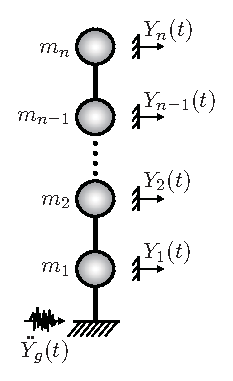
\includegraphics[width=0.2\textwidth] {figure/2-3a.eps}
   \label{fig:2-3a}
 }\hfill
 \subfigure[Separation of whole structure]{
   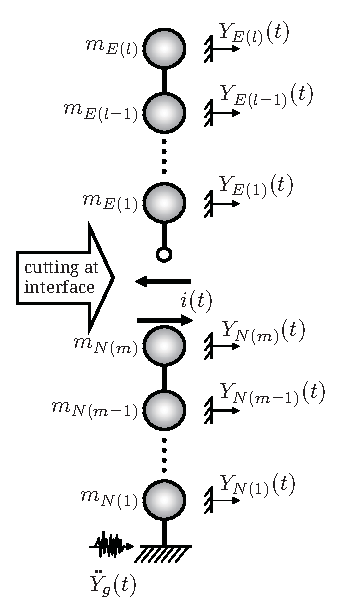
\includegraphics[width=0.3\textwidth] {figure/2-3b.eps}
   \label{fig:2-3b}
 }\hfill
 \subfigure[Experimental and numerical substructure]{
   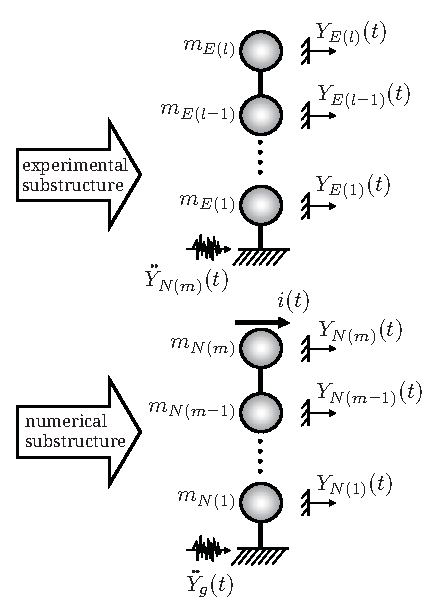
\includegraphics[width=0.4\textwidth] {figure/2-3c.eps}
   \label{fig:2-3c}
 }
\caption{Concept of the proposed method}
\label{fig:2-3}
\end{figure}

It is obvious from Eq.~\eqref{eq:2-7} that the absolute acceleration of the top story of the numerical substructure acts as the ground acceleration of the experimental substructure given by Eq.~\eqref{eq:2-3}. This condition is physically realized by synchronizing the shaking table motion with the absolute acceleration of the top story of the numerical substructure. Besides, the first element of the external force vector in Eq.~\eqref{eq:2-8} means the interface force acting on the top story of the numerical substructure. This interface force, which is denoted by $i(t)$ from now on, is produced by the damping and restoring forces of the first story in the upper experimental substructure and rewritten as follows.

\begin{equation}\label{eq:2-9}
i(t)=c_{E(1)}\left(\dot{Y}_{E(1)}-\dot{Y}_{N(m)}\right)+k_{E(1)}\left(Y_{E(1)}-Y_{N(m)}\right)
\end{equation}

As a result, the numerical substructure, of which equation of motion is given by Eq.~\eqref{eq:2-4}, is subjected to both the interface force at the top story and the ground motion at the base. The boundary condition and external load of each substructure are illustrated in Figure~\ref{fig:2-3c}.


\subsubsection{Measurement of the interface force}

In this section, the interface force, $i(t)$, which should be fed-back to the numerical substructure for calculating the interface acceleration, is indirectly measured by the accelerometers attached on the experimental substructure, as shown in Figure~\ref{fig:2-2}. Dynamic equilibrium in the experimental substructure is applied to derive the interface force using acceleration response measurement of the experimental substructure. As shown in Figure~\ref{fig4:dynamic}, dynamic equilibrium in the experimental substructure is established between the interface force acting at its base and the resultant of its inertial forces, because internal forces between each story are canceled with each other. This relation can be derived in another way. First, the dotted parts are shown in Eq.~\eqref{eq:2-5} are moved to the right side of Eq.~\eqref{eq:2-3}. Then the relation of Eq.~\eqref{eq:2-9} is applied to the right side. Finally, the summation of $l$ simultaneous equations for each side gives following expression of the interface force, $i(t)$.

\begin{equation}\label{eq:2-10}
i(t)=-\sum_{i=1}^{l}m_{E(i)}\ddot{Y}_{E(i)}
\end{equation}

Eq.~\eqref{eq:2-10} physically implies that the interface force, which is required as an input data of the numerical substructure, can be calculated using the measured acceleration responses of the experimental substructure.

\begin{figure}[ht]
\centering
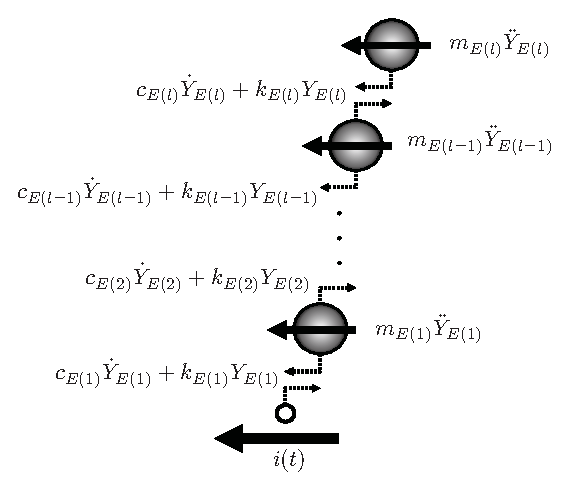
\includegraphics[width=0.6\textwidth] {figure/2-4.eps}
\caption{Dynamic equilibrium in experimental substructure}
\label{fig4:dynamic}
\end{figure}

\subsubsection{Calculation of the numerical substructure}
The calculation of the numerical substructure shown in Figure~\ref{fig:2-2} means on-line time history analysis of the Eq.~\eqref{eq:2-4} that represents the dynamic equilibrium of the numerical substructure shown in Figure~\ref{fig:2-3c}. To integrate this analysis procedure with shaking table control process implemented on a digital computer, Eq.~\eqref{eq:2-4} is transformed into state-space equations. The state-space equations, of which the output is the absolute accelerations of the numerical substructure, are given by the following equations in the continuous time domain.

\begin{equation}\label{eq:2-11}
\begin{aligned}
\matr{\dot{z}}(t)=\matr{A}\matr{z}(t)+\matr{B}\matr{u}(t)\\
\matr{O}(t)=\matr{C}\matr{z}(t)+\matr{D}\matr{u}(t)
\end{aligned}
\end{equation}

where, $\matr{z}(t)$ is the $2m \times 1$ vector of state variables composed of the relative displacement and velocity of the numerical substructure. $\matr{u}(t)$ is the $2 \times 1$ vector of input variables given by $\left\{i(t),\ddot{Y}_{g}(t)\right\}^{\top}$, in which the interface force, $i(t)$, is fed-back from the experimental substructure using Eq.~\eqref{eq:2-10}. $\matr{O}(t)$ is the $m \times 1$ vector of the output composed of the absolute accelerations of the numerical substructure.  The system matrices $\matr{A}$, $\matr{B}$, $\matr{C}$ and $\matr{D}$ have the dimension of $2m \times 2m$, $2m \times 2$, $m \times 2m$ and $m \times 2$, respectively, and are expressed as

\begin{align}
\matr{A}=&\begin{bmatrix} \matr{0}_{m\times m}&\matr{I}_{m\times m}\\-\matr{M}_{N}^{-1}\matr{K}_{N}&-\matr{M}_{N}^{-1}\matr{C}_{N} \end{bmatrix} \label{eq:2-12} \\
\matr{B}=&\begin{bmatrix} \matr{0} & \matr{0} \\ \matr{M}_{N}^{-1}\matr{b}&\matr{-1} \end{bmatrix} \label{eq:2-13} \\
\matr{C}=&\begin{bmatrix} -\matr{M}_{N}^{-1}\matr{K}_{N} & -\matr{M}_{N}^{-1}\matr{C}_{N} \end{bmatrix}\label{eq:2-14} \\
\matr{D}=&\begin{bmatrix} \matr{M}_{N}^{-1}\matr{b} & \matr{0} \end{bmatrix} \label{eq:2-15}
\end{align}

where, $\matr{0}$ and $\matr{I}$ are $m \times m$ zero and unit matrices, respectively, and $\matr{0}$ and $\matr{-1}$ are an $m \times 1$ vector of $0$ and an $m \times 1$ vector of $-1$, respectively. $\matr{b}$ is an $m \times 1$ vector given by $\left\{1, 0, ..., 0 \right\}^{\top}$. Eq.~\eqref{eq:2-11} with the inputs of the interface force and ground motion is incorporated in the `Calculating' part shown in Figure~\ref{fig:2-2}, and produces the absolute acceleration responses of the numerical substructure on-line. Among those acceleration responses, the one corresponding to the top story is utilized as the reference signal to operate shaking table.

\subsection{Numerical Substructure}
For the verification experiment of the proposed methodology, the object structure is assumed to be a five-story shear type building structure, of which two upper stories are assumed to be the experimental substructure as shown in Fifure~\ref{fig:2-8}. As a result, the numerical substructure is the three lower stories of the whole structure. For the construction of the finite element model of the numerical substructure, the inter-story damping and stiffness coefficients of the shear-type experimental substructure are identified based on the measured acceleration responses, and the mass of the two floors are measured directly. The system identification of the experimental substructure is conducted using the command \code{fmincon} in MATLAB\citep{coleman1999optimization}, which uses the interior-reflective Newton method to solve the constrained nonlinear minimization problem \citep{coleman1994convergence,coleman1996interior}. Resulting identified parameters can be summarized as follow.

\begin{equation}\label{eq:2-18}
\begin{aligned}
m_{E(1)}=m_{4}=2.04(kg),~& m_{E(2)}=m_{5}=5.10(kg)\\
k_{E(1)}=k_{4}=45.3(N/m),~& k_{E(2)}=k_{5}=48.5(N/m)\\
c_{E(1)}=c_{4}=0.023(N\cdot s/m),~&c_{E(2)}=c_{5}=0.015(N\cdot s/m)
\end{aligned}
\end{equation}

which correspond to the first and second natural frequencies of $2.5$ and $8.6Hz$, respectively, as given in Table~\ref{tab:2-1}. Figure~\ref{fig:2-10} compares the experimentally obtained transfer functions with numerically computed ones. As shown in Figure~\ref{fig:2-10}, measured transfer functions agree well with those of the corresponding numerical model.

\begin{figure}[ht]
\centering
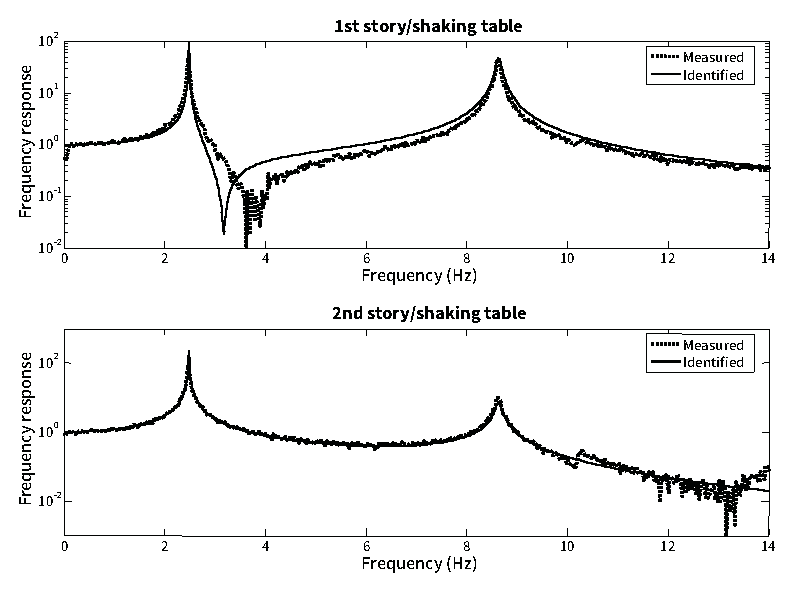
\includegraphics[width=0.8\textwidth] {figure/2-10.eps}
\caption{Comparison of experimental and approximated transfer functions.}
\label{fig:2-10}
\end{figure}

\begin{table}[ht]
\centering
\begin{tabularx}{\textwidth}{@{}X|X|X@{}}
\toprule[1pt]\midrule[0.3pt]
Mode&Frequency components(Hz) observed in the experimental substructure with 2 DOFs&Natural frequencies (Hz) of the whole structure with 5 DOFs\\ \hline
1&1.3&1.3\\
2&2.5&4.2\\
3&4.2&7.1\\
4&7.1&9.4\\
5&8.6&10.8\\ \bottomrule
\end{tabularx}
\caption{Frequencies observed in the time records of the experimental substructure from the test without feedback and the natural frequencies of the assumed whole structure}
\label{tab:2-1}
\end{table}

The structural parameters for the first story of the experimental structure given in Eq.~\eqref{eq:2-18} are applied to all stories of the numerical substructure and summarized as the following:

\begin{align}
i(t)=&-m_{E(1)}\ddot{Y}_{E(1)}(t)-m_{E(2)}\ddot{Y}_{E(2)}(t) \label{eq:2-19} \\
\ddot{Y}_{N(3)}(t)=&-c_{N(3)}\left(\dot{Y}_{N(3)}-\dot{Y}_{N(2)}\right) -k_{N(3)}\left(Y_{N(3)}-Y_{N(2)}\right)+i(t) \label{eq:2-20}
\end{align}

Eq.~\eqref{eq:2-20} means that the interface force, which is produced by the shaking table, is calculated using the two measured absolute accelerations of the experimental substructure. Then, the interface acceleration is calculated from the numerical substructure expressed by Eq.~\eqref{eq:2-11}. Figure~\ref{fig:2-11} represents the block diagram of the entire substructuring testing system including the numerical substructure marked by the shaded area. In Figure~\ref{fig:2-11}, the ground acceleration, $\ddot{Y}_{g}$, is not a measured signal but an input data prescribed by a user. Finally, the shaking table motion is controlled using the inverse transfer function of Eq.~\eqref{eq:2-17} to minimize the errors between the interface acceleration computed as the third story absolute acceleration of the numerical substructure, $\ddot{Y}_{N(3)}$, and the actual shaking table acceleration. Therefore, the shaking table itself works as the interface node of Figure~\ref{fig:2-3b} and excites the upper experimental substructure. In the actual implementation of the shaking table test, the continuous filters included in Figure~\ref{fig:2-11} are converted into discrete filters with a time step of 0.01 sec.

\begin{figure}[ht]
\centering
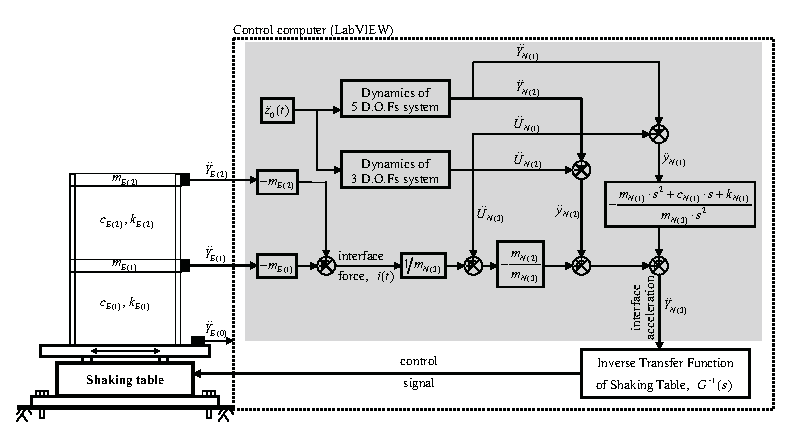
\includegraphics[width=0.8\textwidth] {figure/2-11.eps}
\caption{Block diagram of the integrated controller for the substructuring testing system.}
\label{fig:2-11}
\end{figure}







%!TEX encoding = UTF-8 Unicode
\section{Hybrid Testing Method for the Performance Evaluation of a Tuned Liquid Damper}% hybrid testing method for the Performance Evaluation of a Tuned Liquid Column Damper
\label{chap:3}

In this section, the vibration control effect of a TLD for a building structure excited by earthquake load is experimentally evaluated through the hybrid testing method. The hybrid testing method does not require a physical building structural model in performing the experiment of a TLD–structure interaction system, and it only uses a TLD which is known to have strong nonlinearity dependent on response amplitude, excitation frequency, and depth to length ratio\citep{yu1999non}. The structural responses of the interaction system are calculated numerically in real time using the analytical structural model with the excitations of measured control force, user-defined base earthquake loads, and its state space realization incorporated in the integrated controller of the shaking table. Also, in order to minimize the distortion of the acceleration of the shaking table, the inverse transfer function of the shaking table is identified, and its state space realization is implemented in the shaking table controller. The motion of shaking table behaves both the controlled and uncontrolled absolute acceleration of the TLD mounted floor by modulating the feedback gain of the shear force measured by the load cell installed between the TLD and the shaking table. Comparison between the structural responses obtained by the hybrid testing method and the conventional shaking table test of a single story steel frame with TLD is made in order to verify the accuracy of the hybrid testing method and the uncontrolled and TLD-controlled structural responses of a three-story structure are obtained by the hybrid testing method in both time and frequency domains.

\subsection{Hybrid Testing Method with TLD}
Figure~\ref{fig:3-1} depicts the conceptual illustrations of the hybrid testing method for an n-degrees-of-freedom structural model which is excited by base acceleration and has a tuned liquid damper at its top story. First, the whole control system is separated into the lower part structure, and the upper part TLD and the interaction force between the structure and TLD are considered. The TLD with the interacting force at its bottom is physically tested, and the response of the structure with interacting force at the top floor and the base acceleration is numerically calculated by using the computer controlling the motion of the shaking table. Measurement of interacting force is easily accomplished by installing a shear-type load-cell at the bottom of the TLD, as shown in Figure~\ref{fig:3-1}. TLD-generated shear force is fed back to the control computer. With this fed-back interacting force, the structural response of the story, where a TLD is installed, is calculated using the numerical part. The shaking table excites the upper TLD according to this calculated response. This process is carried out on real-time.

\begin{figure}[ht]
\centering
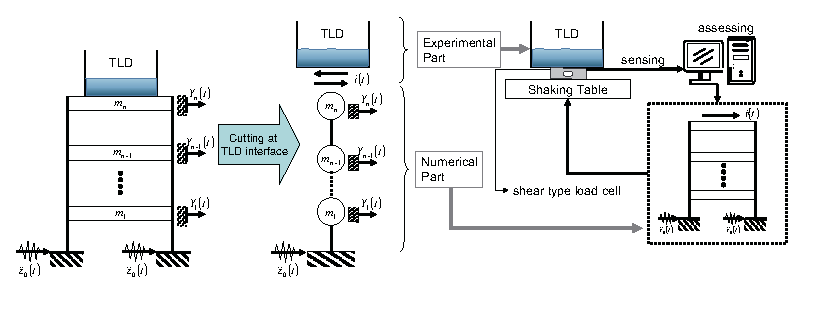
\includegraphics[width=\textwidth] {figure/3-1.eps}
\caption{Conceptual view of the hybrid shaking table test}
\label{fig:3-1}
\end{figure}

The numerical part with $n-$DOFs, which is subjected to the excitations of the measured control force, $i_{e}(t)$, and the input acceleration, $\ddot{z}_{0}(t)$, at its top and bottom, respectively, as enclosed in dotted line in Figure~\ref{fig:3-1}, is calculated by

\begin{equation}\label{eq:3-1}
\matr{M}\matr{\ddot{Y}}_{i}(t) + \matr{C}\matr{\dot{Y}}_{i}(t) + \matr{K}\matr{Y}_{i}(t) = \matr{p}(t)
\end{equation}

where, $\matr{Y}_{i}(t)$ is the absolute displacement at the $i$th$\left(i=1\rightarrow n\right)$ story, and the location vector of external forces with the length of $n$, $\matr{p}(t)$  equals to $\left\{ -i_{e}(t),0,...,0,c_{1}\dot{z}_{0}(t)+k_{1}z_{0}(t)\right\}^{\top}$, in which subscript ``$e$'' denotes the ``\textit{experimentally}'' measured interacting force. Also, the structural mass, damping and stiffness matrices are represented by

\begin{equation}\label{eq:3-2}
\begin{aligned}
\matr{M}=\begin{bsmallmatrix}m_{n}&&&\\&m_{n-1}&&\\&&\ddots&m_{1}\end{bsmallmatrix},
\matr{C}=\begin{bsmallmatrix}c_{n}&-c_{n}&&\\-c_{n}&c_{n}+c_{n-1}&-c_{n-1}&\\ &\ddots&\ddots&\ddots\\&&-c_{2}&c_{2}+c_{1}\end{bsmallmatrix},\\
\matr{K}=\begin{bsmallmatrix}k_{n}&-k_{n}&&\\-k_{n}&k_{n}+k_{n-1}&-k_{n-1}&\\ &\ddots&\ddots&\ddots\\&&-k_{2}&k_{2}+k_{1}\end{bsmallmatrix}
\end{aligned}
\end{equation}

To calculate the numerical part such as Eq.~\eqref{eq:3-2} by a control computer on real-time, it is transformed into the state-space representation given by

\begin{equation}\label{eq:3-3}
\begin{aligned}
\matr{\dot{z}}(t)&=\matr{A}_{c}\matr{z}(t)+\matr{B}_{c}\matr{u}(t)\\
\matr{O}(t)&=\matr{C}_{c}\matr{z}(t)+\matr{D}_{c}\matr{u}(t)
\end{aligned}
\end{equation}

where, the state variable vector, $\matr{z}(t)$, with the length of $2n$ comprises the state variables, $\left\{\matr{y}_{i}(t),\matr{\dot{y}}_{i}(t)\right\}^{\top}$, in which the structural relative displacement, $\matr{y}_{i}(t)$, equals to $\matr{Y}_{i}(t)-z_{0}(t)$. The input vector, $\matr{u}(t)$, with the length of 2 consists of $\left\{-i_{e}(t), \ddot{z}_{0}\right\}^{\top}$. The output vector, $\matr{O}(t)$, with the length of $n$ corresponds to the structural absolute acceleration, $\matr{\ddot{Y}}_{i}(t)$, itself. The matrices $\matr{A}_{c}$, $\matr{B}_{c}$, $\matr{C}_{c}$ and $\matr{D}_{c}$ with the sizes of $2n \times 2n$, $2n \times 2$, $n \times 2n$ and $n \times 2$, respectively, are expressed as the following Eqs.~\eqref{eq:3-4}-\eqref{eq:3-7}.

\begin{align}
\matr{A}_{c}&=\begin{bmatrix} \matr{0}_{m\times n}&\matr{I}_{m \times n}\\-\matr{M}^{-1}\matr{K}&-\matr{M}^{-1}\matr{C}\end{bmatrix} \label{eq:3-4}\\
\matr{B}_{c}&=\begin{bmatrix} \matr{0}_{n\times 1}&\matr{0}_{n\times 1}\\ \matr{M}^{-1}\matr{b}&\matr{-1}\end{bmatrix} \label{eq:3-5}\\
\matr{C}_{c}&=\begin{bmatrix} -\matr{M}^{-1}\matr{K}&-\matr{M}^{-1}\matr{C}\end{bmatrix} \label{eq:3-6}\\
\matr{D}_{c}&=\begin{bmatrix} \matr{M}^{-1}\matr{b}&\matr{0}_{m \times 1}\end{bmatrix} \label{eq:3-7}
\end{align}


%!TEX encoding = UTF-8 Unicode
\section{Hybrid testing method for the Performance Evaluation of a Tuned Liquid Column Damper}
\label{chap:4}

The tuned liquid column damper has received the attention of researchers as a type of auxiliary mass system\citep{samali1998wind}. TLCD has the control characteristics similar to that of tuned mass damper, which is one of most frequently used dampers for vibration control. Since the viscosity term in the governing equation of motion of TLCD is a function of the absolute value of liquid velocity, the equation is nonlinear, and the dynamic characteristics of TLCD depend on the magnitude and the characteristics of excitation forces and the corresponding structural responses of the floor at which TLCD is installed\citep{yalla2001liquid}.
In this section, the vibration control effect of a TLCD for a building structure excited by earthquake load is experimentally evaluated through the hybrid testing method. The hybrid testing method does not require a physical building structural model in performing the experiment of a TLCD-structure interaction system, and it only uses a TLCD. The structural responses of the interaction system are calculated numerically in real time using the analytical structural model with the excitations of measured control force, user-defined base earthquake loads, and its state space realization incorporated in the integrated controller of the shaking table. Also, in order to minimize the distortion of the acceleration of the shaking table, the inverse transfer function of the shaking table is identified, and its state space realization is implemented in the shaking table controller. The shaking table behaves as the absolute acceleration of the TLCD mounted floor by calculating the fed back signal of the shear force signal measured by the load cell positioned between the TLCD and plate of the shaking table. Comparison results between the structural responses obtained by the hybrid testing method and the conventional shaking table test of a single story steel frame with TLCD are made to verify the accuracy of the hybrid testing method in both time and frequency domains.

\subsection{Hybrid Testing Method with TLCD}
Figure~\ref{fig:4-1} shows the conceptual view of the experiment. The whole structural control system, which a TLCD was installed onto the structural model with n-degrees-of-freedom at its top story, is separated, and as the result of that, the force interacts at their interface. The upper part of TLCD with the interacting force at its bottom is physically tested and the lower part of the structural model with the interacting force and the input motion at its top story and base, respectively, is numerically calculated within the computer to control the motion of shaking table. For the experimental implementation, interacting or control force generated by a TLCD, which is observed from a load-cell, is fed back to the control computer. With the fed-back interacting force, the structural response of the story, where a TLCD is incorporated, is calculated from the numerical part. The shaking table excites the upper TLCD with this calculated response. These processes are carried out on real-time.

\begin{figure}[ht]
\centering
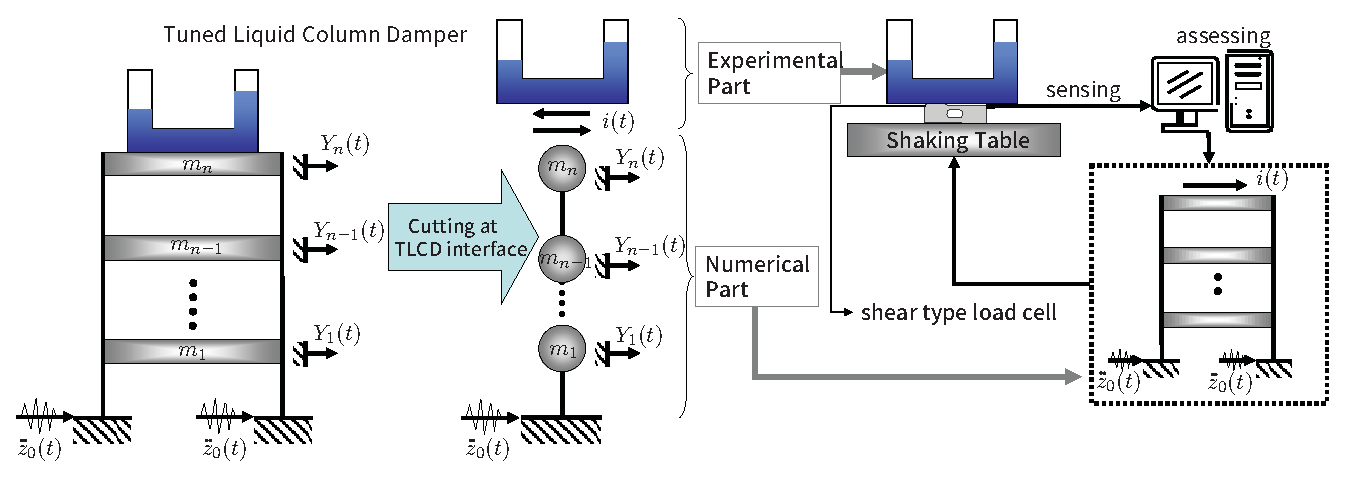
\includegraphics[width=1\textwidth] {figure/4-1.eps}
\caption{Concept of the hybrid testing method (TLCD)}
\label{fig:4-1}
\end{figure}

Of theses procedures, the numerical part with $n$-DOFs, which is subjected to the excitations of the experimentally measured control force, $i_{e}(t)$, and the input acceleration, $\ddot{z}_{0}(t)$, at its top and bottom, respectively, as enclosed in dotted line in Figure~\ref{fig:4-1}, is calculated by

\begin{equation}\label{eq:4-1}
\matr{M}\matr{\ddot{Y}}_{i}(t)+\matr{C}\matr{\dot{Y}}_{i}(t)+\matr{K}\matr{Y}_{i}(t)=\matr{p}(t)
\end{equation}

where, $\matr{Y}_{i}(t)$ is the absolute displacement at the $i$th$\left(i=1\rightarrow n\right)$ story, and the location vector of external forces with the length of $n$, $\matr{p}(t)$  equals to $\left\{ -i_{e}(t),0,...,0,c_{1}\dot{z}_{0}(t)+k_{1}z_{0}(t)\right\}^{\top}$, in which subscript ``$e$'' denotes the ``\textit{experimentally}'' measured interacting force. Also, the structural mass, damping and stiffness matrices are represented by

\begin{equation}\label{eq:4-2}
\begin{aligned}
\matr{M}=\begin{bsmallmatrix}m_{n}&&&\\&m_{n-1}&&\\&&\ddots&m_{1}\end{bsmallmatrix},
\matr{C}=\begin{bsmallmatrix}c_{n}&-c_{n}&&\\-c_{n}&c_{n}+c_{n-1}&-c_{n-1}&\\ &\ddots&\ddots&\ddots\\&&-c_{2}&c_{2}+c_{1}\end{bsmallmatrix},\\
\matr{K}=\begin{bsmallmatrix}k_{n}&-k_{n}&&\\-k_{n}&k_{n}+k_{n-1}&-k_{n-1}&\\ &\ddots&\ddots&\ddots\\&&-k_{2}&k_{2}+k_{1}\end{bsmallmatrix}
\end{aligned}
\end{equation}

To calculate the numerical part such as Eq.~\eqref{eq:3-2} by a control computer on real-time, it is transformed into the state-space representation given by

\begin{equation}\label{eq:4-3}
\begin{aligned}
\matr{\dot{z}}(t)&=\matr{A}_{c}\matr{z}(t)+\matr{B}_{c}\matr{u}(t)\\
\matr{O}(t)&=\matr{C}_{c}\matr{z}(t)+\matr{D}_{c}\matr{u}(t)
\end{aligned}
\end{equation}

where, the state variable vector, $\matr{z}(t)$, with the length of $2n$ comprises the state variables, $\left\{\matr{y}_{i}(t),\matr{\dot{y}}_{i}(t)\right\}^{\top}$, in which the structural relative displacement, $\matr{y}_{i}(t)$, equals to $\matr{Y}_{i}(t)-z_{0}(t)$. The input vector, $\matr{u}(t)$, with the length of 2 consists of $\left\{-i_{e}(t), \ddot{z}_{0}\right\}^{\top}$. The output vector, $\matr{O}(t)$, with the length of $n$ corresponds to the structural absolute acceleration, $\matr{\ddot{Y}}_{i}(t)$, itself. The matrices $\matr{A}_{c}$, $\matr{B}_{c}$, $\matr{C}_{c}$ and $\matr{D}_{c}$ with the sizes of $2n \times 2n$, $2n \times 2$, $n \times 2n$ and $n \times 2$, respectively, are expressed as the following Eqs.~\eqref{eq:4-4}-\eqref{eq:4-7}.

\begin{align}
\matr{A}_{c}&=\begin{bmatrix} \matr{0}_{m\times n}&\matr{I}_{m \times n}\\-\matr{M}^{-1}\matr{K}&-\matr{M}^{-1}\matr{C}\end{bmatrix} \label{eq:4-4}\\
\matr{B}_{c}&=\begin{bmatrix} \matr{0}_{n\times 1}&\matr{0}_{n\times 1}\\ \matr{M}^{-1}\matr{b}&\matr{-1}\end{bmatrix} \label{eq:4-5}\\
\matr{C}_{c}&=\begin{bmatrix} -\matr{M}^{-1}\matr{K}&-\matr{M}^{-1}\matr{C}\end{bmatrix} \label{eq:4-6}\\
\matr{D}_{c}&=\begin{bmatrix} \matr{M}^{-1}\matr{b}&\matr{0}_{m \times 1}\end{bmatrix} \label{eq:4-7}
\end{align}

where, $\matr{0}_{n \times n}$ and $\matr{I}_{n \times n}$ are the zero and unit matrices, respectively, with the size of $n\times n$. $\matr{0}_{n\times 1}$ and $\matr{-1}$ are the vector whose components are $0$ and $-1$, respectively, with the length of $n \times 1$. $\matr{b}$ equal to $\left\{1,0,...,0\right\}^{\top}$ with the length of $n \times 1$.


%!TEX encoding = UTF-8 Unicode
\section{Hybrid Testing Method for the Performance Evaluation of a Tuned Liquid Mass Damper}
\label{chap:5}

In previous study\citep{heo2009performance}, a new control device, which is called tuned liquid mass damper (TLMD), was developed and discussed in this section. The dynamic characteristics of a TLMD used in this study are that its mass is composed of both a mass of TLCD frame itself and that of liquid in a tank. Natural rubber columns were used to substitute the stiffness of a TMD. Therefore, a TLMD operates as a TLCD in one direction and behaves as a TMD in the other orthogonal direction. 

In this section, the control performance of the proposed TLMD for reducing bidirectional responses of building structures is experimentally verified through both a conventional structural testing method and hybrid testing method. First, the control performance of a TLMD is evaluated by forced vibrating sinusoidal signal to an experimental prototype which is composed of both a TLMD and a  building structure. Then, the hybrid testing method is performed to evaluate the performance of a TLMD, in which the building structural model is used as a numerical part, and the TLMD is experimentally tested.

\subsection{Developed TLMD Model}
Figure~\ref{fig:5-1} shows the plan view of the TLMD used in this study. The bidirectional TLMD would be installed in the POSCO New Songdo City Tower 1A in Incheon, South Korea with 64 stories and 236 meters in height. An eigenvalue analysis of the tower resulted in $0.182$ and $0.162Hz$ in the $x, y$-directions, respectively, for the first natural frequencies, and $34,000tons$ for the first modal mass. The total mass of the bidirectional TLMD is $600tons$ that results from the effective mass ratio of about $1.76\%$.

The experimental building and TLMD models were manufactured by applying the scaling factors given in Table~\ref{tab:5-1} to the first modal properties of the prototype tower. The building model with the parameters shown in Table~\ref{tab:5-2} was made by applying the scaling factors in Table\ref{tab:5-1} to the prototype building. Applying the scale $1/\sqrt{20}$ in frequency to the natural frequencies of a prototype model, $0.182$ and $0.162Hz$, gives $0.82$ and $0.73Hz$ in the $x-$ and $y-$directions, respectively. Also, the mass of a building structure is reduced by $4,250kg$. The stiffness of a building model is calculated to be $4250(kg)\times \left(2\pi \times 0.82(Hz)\right)^{2}\cong 110 000(N/m)$ in the $x-$direction and $4250(kg)\times \left(2\pi \times 0.73(Hz)\right)^{2} \cong 89,000(N/m)$ in the $y-$direction, respectively.

\begin{figure}[ht]
\centering
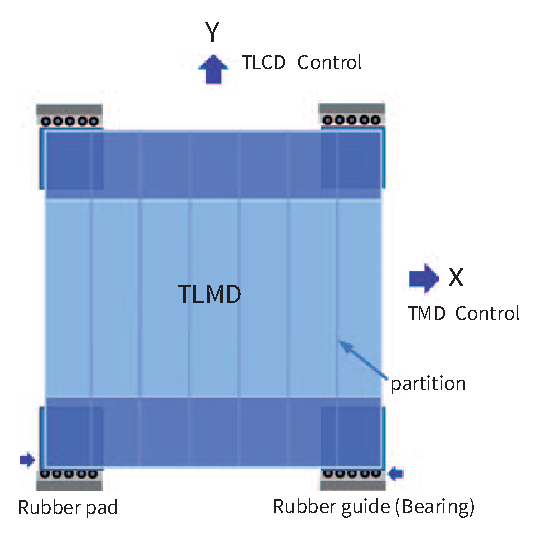
\includegraphics[width=0.8\textwidth] {figure/5-1.eps}
\caption{Concept of a TLMD}
\label{fig:5-1}
\end{figure}

\begin{table}[ht]
\centering
\begin{tabularx}{\textwidth}{@{}X|X|X@{}}
\toprule[1pt]\midrule[0.3pt]
Quantity & Dimension & Scaling factor\\ \hline
Length & $L$ & $1:20$\\
Mass & $M$ & $1:20^{3} = 1:8000$\\
Frequency (Hz) & $T^{-1}$ & $1:1/\sqrt{20} = 1:0.223$\\
Acceleration & $LT^{-2}$ & $1:1$\\
\bottomrule
\end{tabularx}
\caption{Similitude law applied to TLMD model}
\label{tab:5-1}
\end{table}

\begin{table}[ht]
\centering
\begin{tabularx}{\textwidth}{@{}X|X|X@{}}
\toprule[1pt]\midrule[0.3pt]
Design parameter & $y-$direction & $x-$direction\\ \hline
Siffness (N/m) & $88,000$ & $110,000$\\
Frequency (Hz) & $0.73$ & $0.82$\\
Mass (kg) & $4,250$ & $4,250$\\
\bottomrule
\end{tabularx}
\caption{Design parameters of the building model}
\label{tab:5-2}
\end{table}

\begin{table}[ht]
\centering
\begin{tabularx}{\textwidth}{@{}X|X|X@{}}
\toprule[1pt]\midrule[0.3pt]
Design parameters & TLCD control direction & TMD control direction\\ \hline
Siffness or liquid length & $0.98m$ (liquid length) & $1990N/m$ (stiffness)\\
Frequency (Hz) & $0.73$ & $0.82$\\
Mass (kg) & $35$ & $75$\\
\bottomrule
\end{tabularx}
\caption{Design parameters of a TLMD model}
\label{tab:5-3}
\end{table}

As shown in Table~\ref{tab:5-3}, it is obvious that the natural frequencies of a TLMD tune to those of a building structure in the TMD$(x)$ and TLCD$(y)$-control directions, respectively. The masses of a TLMD with the ratios of $1.8$ and $0.8\%$ to the mass of a building model become $75kg$ in the TMD-control and $32kg$ in the TLCD-control directions, respectively. The stiffness of rubber columns used in a TMD, $k$, and the liquid length of a TLCD, $L$, are determined by

\begin{align}
k&=m\left(2\pi f_{m}\right)^{2} \label{eq:5-1} \\
L&=\frac{2g}{\left(2\pi f_{L}\right)^{2}} \label{eq:5-2}
\end{align}

where $m$ and $f_{m}$ are the mass and the tuned frequency of a TLCD, respectively, in the TMD-control direction. $g$ and $f_{L}$ are the gravity acceleration and the tuned frequency of the TLCD, respectively, in the TLCD-control direction. With these relations, the final parameters of a TLMD are shown in Table~\ref{tab:5-3}.








\clearpage
\section{Design of Experimental Controller}
\subsection{Experimental System for Substructurubg Technique}

The experimental system is shown in Figure~\ref{fig:2-5} and \ref{fig:2-6} was equipped in Seismic Retrofitting \& Remodeling Research Center at the Dankook University, Seoul, Korea. The test structure (the experimental substructure) used in this experiment is a two-story steel frame with a single bay. The height and width of the experimental substructure are 1.0 and 0.6 m, respectively. The first floor mass, $m_{E(1)}$, and the second floor mass, $m_{E(2)}$, are 2.04 and 5.10 kg, respectively. The experimental substructure is excited by a uni-axial shaking table. The accelerometers are attached to each floor of the experimental substructure to measure its absolute floor acceleration responses. Additionally, an accelerometer is placed on the shaking table to monitor its motion. The data acquisition and implementation of the digital shaking table controller are performed using a real-time digital signal processor (DSP). The major task of the data acquisition board is to carry out the analog-to-digital (A/D) conversion of the measured acceleration data and the digital-to-analog (D/A) conversion of the reference signal computed by the shaking table controller, which is programmed using LabVIEW \citep{bishop2007labview}. An 8-channel data acquisition system was employed using an NI PCI-6052E board and an NI SC-2345 BNC cable connector as a signal conditioner.

\begin{figure}[ht]
\centering
\includegraphics[width=0.8\textwidth] {figure/2-5.eps}
\caption{Overall view of experimental system}
\label{fig:2-5}
\end{figure}

\begin{figure}[ht]
\centering
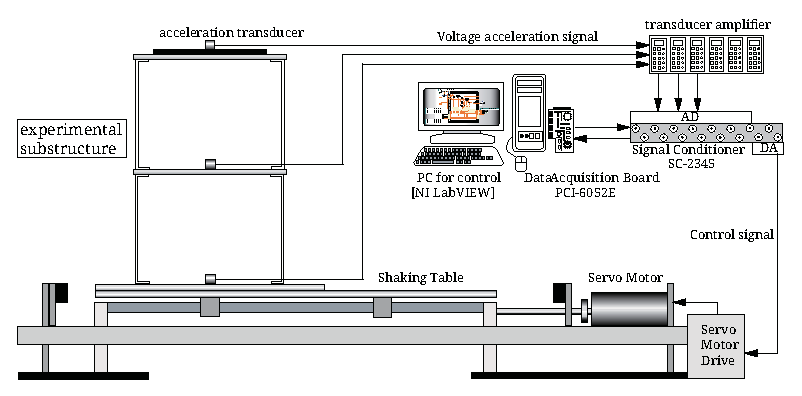
\includegraphics[width=0.8\textwidth] {figure/2-6.eps}
\caption{Schematic diagram of experimental system}
\label{fig:2-6}
\end{figure}

\subsection{Shaking table controller}
The composition of the experimental system is illustrated in Figure~\ref{fig:2-6}. The shaking table shown in Figure~\ref{fig:2-6} moves in accordance with the control signal, which is generated by the control computer and sent through D/A conversion board. In almost every case, the target acceleration signal and actual acceleration produced by the shaking table are different in their amplitudes and phases due to the shaking table dynamics. Therefore, in order to compensate the distortion of the actual shaking table acceleration against the shaking table dynamics existing between the reference signal and the actual measured acceleration of the shaking table, the inverse transfer function of the actual acceleration of shaking table with respect to the command signal generated by the control computer is constructed and implemented in the shaking table control computer as shown in Figure~\ref{fig:2-8}. First, the inverse transfer function, of which amplitude and phase are represented in Figure~\ref{fig:2-7} by the dashed line, is obtained experimentally. Then, the experimental inverse transfer function is approximated by a rational function for its implementation in the control computer. In this verification experiment, the inverse transfer function of the shaking table is approximated using the command \code{invfreqs} in MATLAB \citep{little1992signal}, which adopts the damped Gauss-Newton method for the iterative search to minimize the sum of the squared error between the measured and the desired frequency response points\citep{dennis1983numerical}. The approximation result is given by the following 5-th order linear filter and compared with the experimental one in Figure~\ref{fig:2-7}. 

\begin{figure}[ht]
\centering
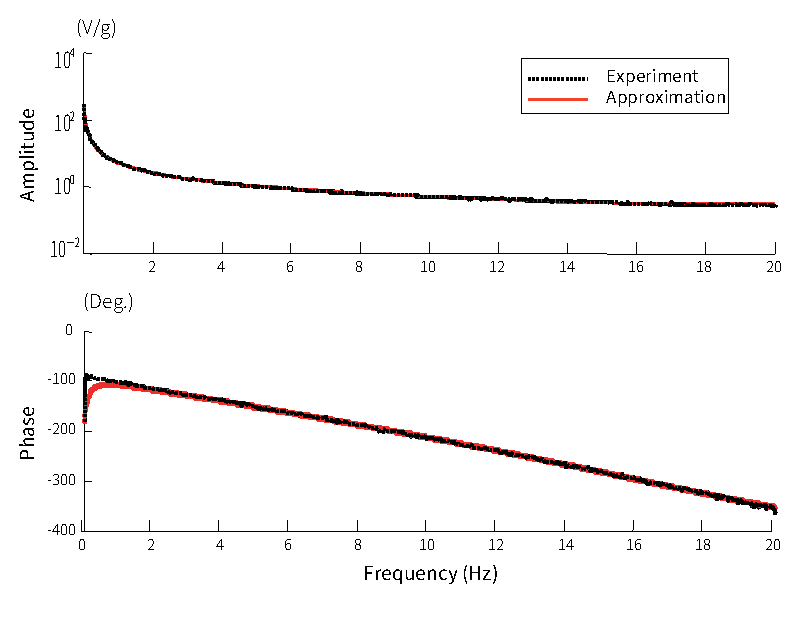
\includegraphics[width=0.8\textwidth] {figure/2-7.eps}
\caption{Inverse transfer function of shaking table}
\label{fig:2-7}
\end{figure}

Inverse transfer function, Eq.~\eqref{eq:2-16}, corresponds to the shaking table controller of Figure~\ref{fig:2-2}. 

\begin{equation}\label{eq:2-16}
G^{-1}(s) = \frac{0.6s^5 + 94s^4 + 10746s^3 + 498200s^2 + 167124s + 108216}{s^5 + 204s^4 + 15900s^2 + 8252s^2 + 4676s + 405}
\end{equation}

\begin{figure}[ht]
\centering
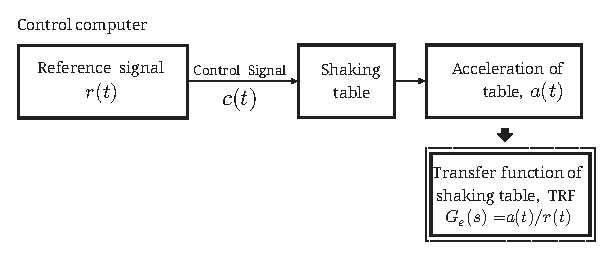
\includegraphics[width=0.8\textwidth] {figure/5-13.eps}
\caption{Definition of the transfer function of shaking table}
\label{fig:5-13}
\end{figure}

\begin{figure}[ht]
\centering
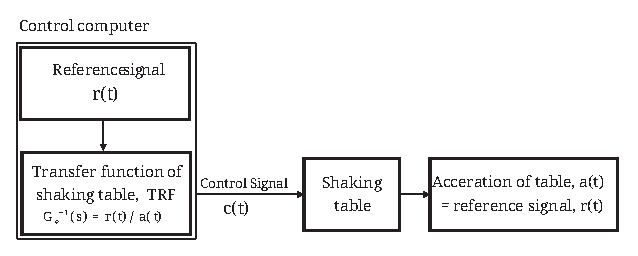
\includegraphics[width=0.8\textwidth] {figure/5-14.eps}
\caption{Compensation using the inverse transfer function of shaking table}
\label{fig:5-14}
\end{figure}

For the implementation in the digital computer, Eq.~\eqref{eq:2-16} is realized into the following state equation.

\begin{equation}\label{eq:2-17}
\begin{aligned}
\matr{\dot{x}}_{c} = \matr{A}_{c}\matr{x}_{c} + \matr{B}_{c}r_{c}\\
y_{c}=\matr{C}_{c}\matr{x}_{c}+D_{c}r_{c}
\end{aligned}
\end{equation}

where, $\matr{x}_{c}$, $r_{c}$ and $y_{c}$ is the state vector, the reference signal, the control signal of the shaking table controller, respectively. $\matr{A}_{c}$, $\matr{B}_{c}$, $\matr{C}_{c}$ and $D_{c}$ is the $5\times5$ state matrix, the $5\times1$ reference signal influence matrix, the $1\times5$ output matrix and the coupling coefficient between the reference and control signal.

\begin{figure}[ht]
\centering
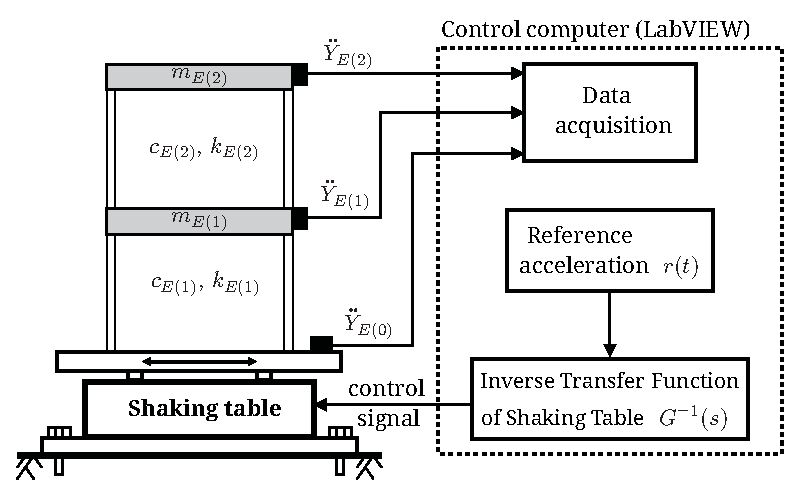
\includegraphics[width=0.8\textwidth] {figure/2-8.eps}
\caption{Flow chart of the experimental system controller}
\label{fig:2-8}
\end{figure}

In order to verify the performance of the shaking table controller, a down-scaled El Centro earthquake is input to the inverse transfer function of the shaking table. Then, the corresponding acceleration of the shaking table is measured. Figure~\ref{fig:2-9} compares the reference acceleration with the corresponding measured acceleration of the shaking table. It is observed that they agree well with each other.

\begin{figure}[ht]
\centering
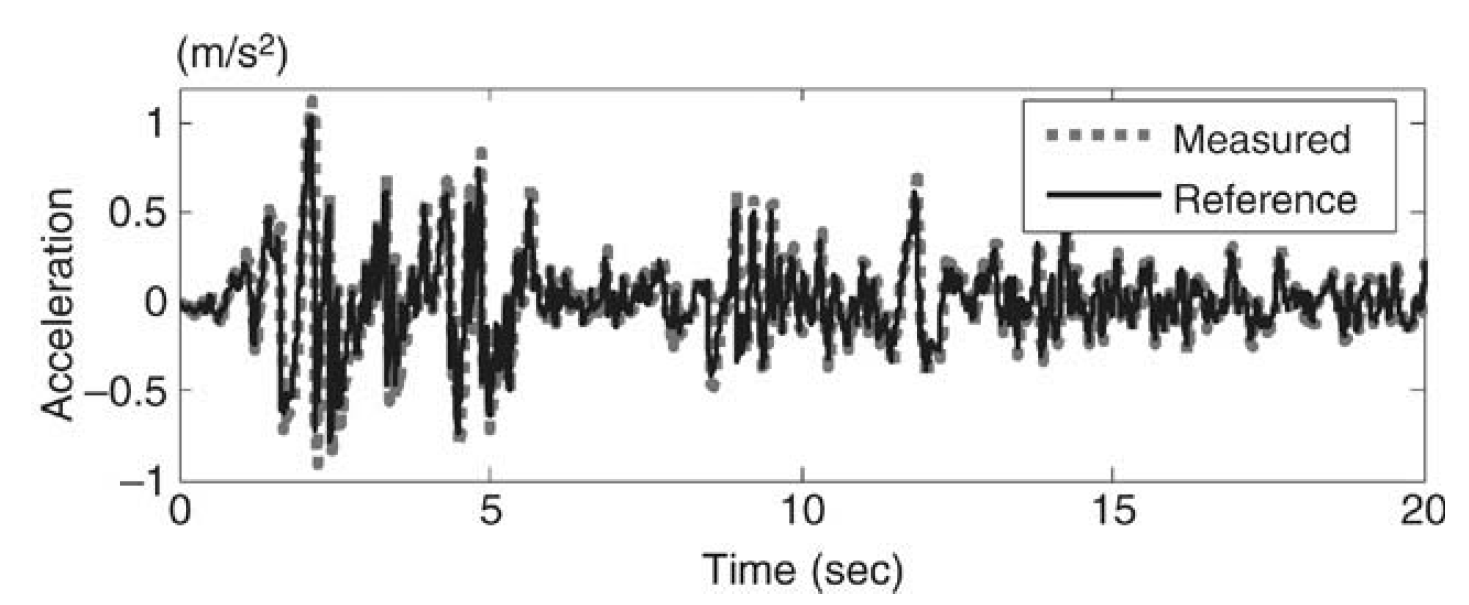
\includegraphics[width=0.8\textwidth] {figure/2-9.png}
\caption{Compensation result for the dynamic characteristic of shaking table}
\label{fig:2-9}
\end{figure}






\subsection{Experimental System for Hybrid Testing of Building with TLD}
\subsubsection{Experimental setup}

In order to experimentally verify the hybrid testing method, an experimental system shown in Figure~\ref{fig:3-2} was set up in Seismic Retrofitting \& Remodeling Research Center at the Dankook University, Seoul, Korea. The TLD was uniaxially excited by the shaking table on which it was mounted. The shear-type load-cell was inserted between the TLD and the shaking table to measure the base shear force yielded by the horizontal motion of the TLD during the test. Also, an accelerometer was attached to the shaking table to monitor its motion.

\begin{figure}[ht]
\centering
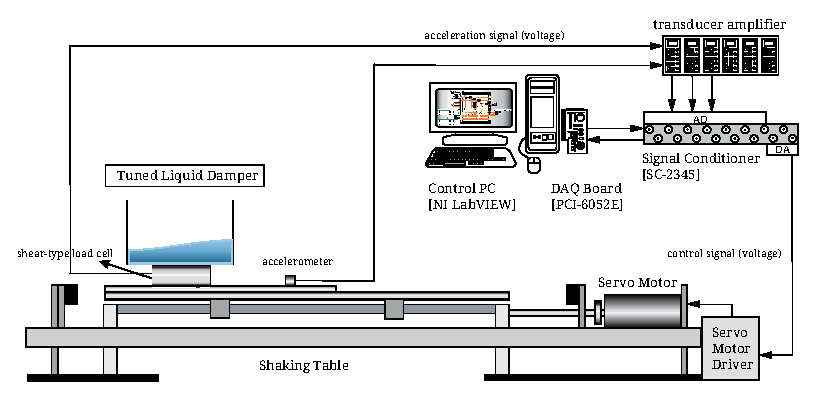
\includegraphics[scale =1] {figure/3-2.eps}
\caption{Schematic diagram of experimental set-up}
\label{fig:3-2}
\end{figure}

\subsubsection{Integrated Controller of the Numerical Structural Model and the Shaking Table}
The numerical structural model and the shaking table dynamics discussed in the previous subsections are integrated into the controller to implement the hybrid testing method. Figure~\ref{fig:3-3} illustrates the block diagram of the hybrid testing method. In the figure, the absolute acceleration is produced by the numerical structural model of Eq.~\eqref{eq:3-3} with two inputs of the measured interacting force, $i_{e}(t)$, and not the measured but the prescribed earthquake record signal, $\ddot{z}_{0}(t)$, as marked by the shaded area. The motion of the shaking table is driven by the controller using the inverse transfer function to minimize the error between the absolute acceleration, $\ddot{Y}_{n}(t)$, calculated as the top story response of the structure and the actual shaking table acceleration, $\ddot{Y}_{e}(t)$. Accordingly, the shaking table itself behaves as the top story of the structure, at which a TLD is installed, and excites the upper TLD that should be physically tested.

\begin{figure}[ht]
\centering
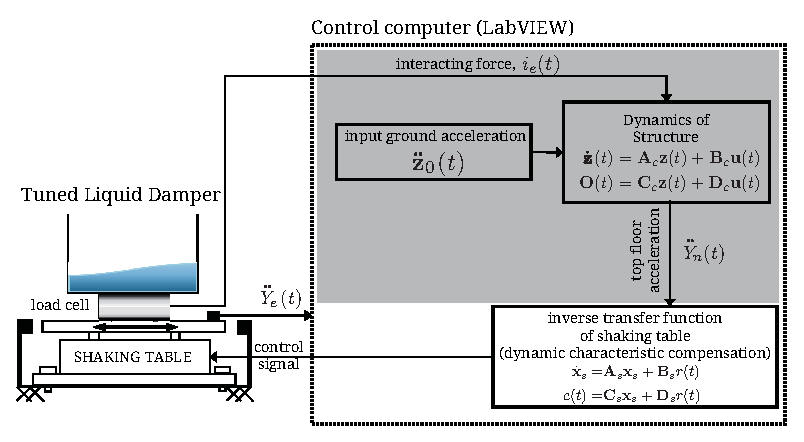
\includegraphics[scale =1] {figure/3-3.eps}
\caption{Block diagram of the integrated controller for the hybrid testing system.}
\label{fig:3-3}
\end{figure}









\subsection{Experimental System for Hybrid Testing of Building with TLCD}
The numerical part and the shaking table controller discussed in previous subsections should be integrated into the controller to implement the hybrid testing shown in Figure~\ref{fig:4-1}. Figure~\ref{fig:4-3} illustrates the block diagram for experimentally implementing the testing method. In the figure, the absolute acceleration is produced by the numerical part such as Eq.~\eqref{eq:4-3} with two inputs of the measured interacting force, $i_{e}(t)$, and not the measured but the prescribed earthquake record signal, $\ddot{z}_{0}(t)$, by a user in the control computer, as marked by the shaded area. The motion of shaking table is driven by the controller using the inverse transfer function to minimize the error between the controlled absolute acceleration, $\ddot{Y}_{n}(t)$, calculated as the top story response of structure and the actual shaking table acceleration, $\ddot{Y}_{e}(t)$. Accordingly, the shaking table itself behaves as the top story of structure, at which a TLCD is installed, and excites the upper TLCD that should be physically tested.
To verify the hybrid testing method, firstly the conventional TLCD-structure interaction model shown in Figure~\ref{fig:4-4a} is experimentally implemented. Then, the hybrid test is shown in Figure~\ref{fig:4-4b}, which the structural model in Figure~\ref{fig:4-4a} is incorporated in the numerical calculation of its identified damping and stiffness coefficients and measured mass, is performed for the controlled case. Finally, two results from controlled cases are compared for the experimental verification of the hybrid testing method.

\begin{figure}[ht]
\centering
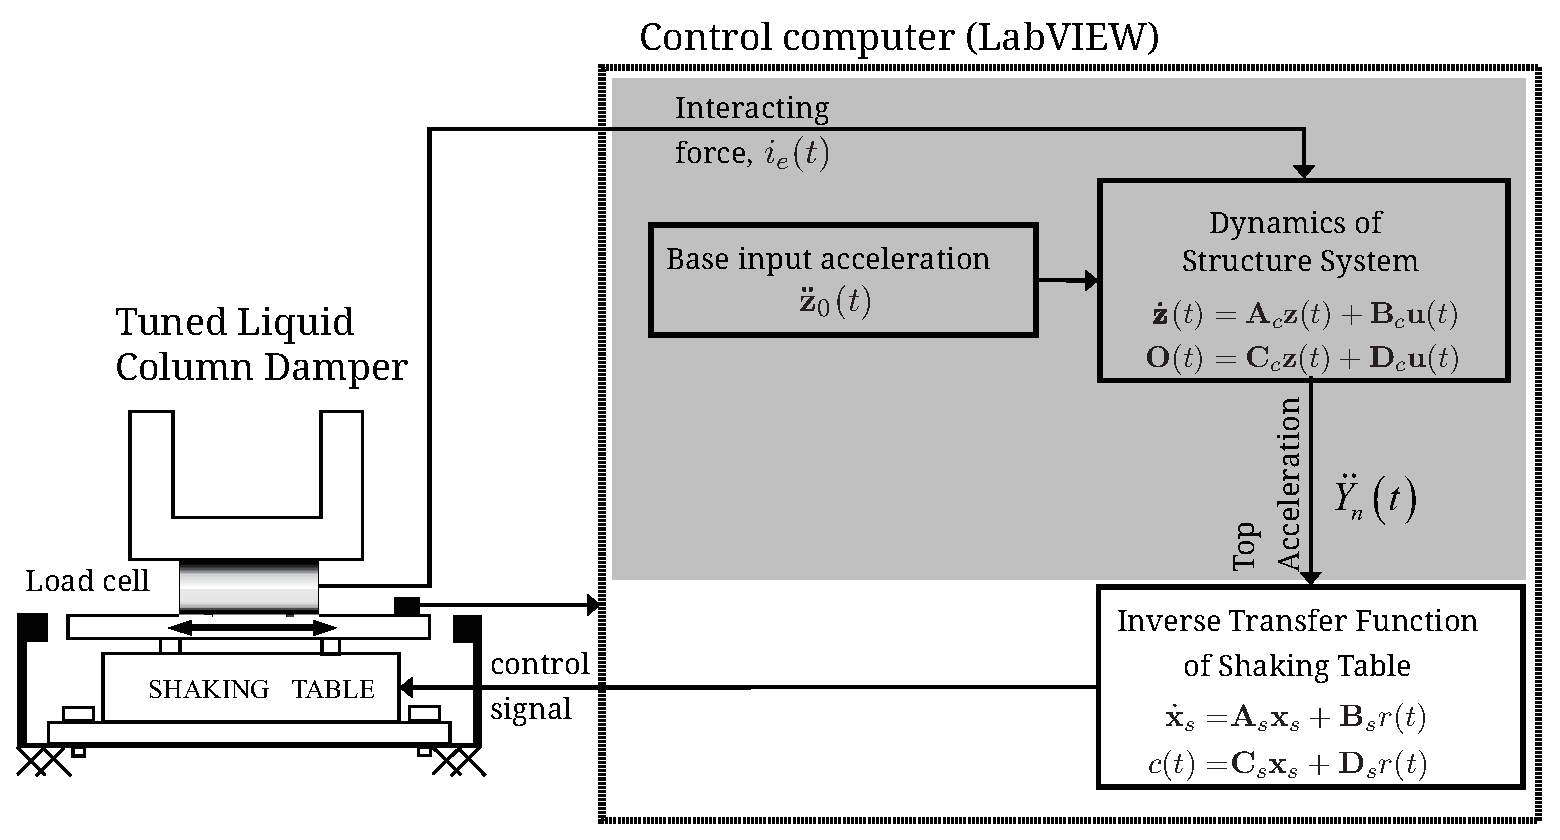
\includegraphics[width=1\textwidth] {figure/4-3.eps}
\caption{Controller for implementing the hybrid testing method}
\label{fig:4-3}
\end{figure}

The only shear-type structural model without the upper TLCD shown in Figure~\ref{fig:4-4a} has the $0.6m$ and $1.0m$ of width and height and $169.7kg$ of measured floor mass. Two records of El Centro and Kobe earthquake waves were excited by the shaking table to measure the absolute structural acceleration. The identification was conducted with measured accelerations of the structure model and the shaking table. The identified parameters have slight differences according to input earthquake waves. The averaged damping, and stiffness coefficients were determined by $14.6N\cdot s/m$ and $9914.3N/m$, respectively, which correspond to $1.23Hz$ of structural natural frequency. The level of water in a TLCD tank was adjusted to sympathize the TLCD frequency to this identified structural one.

\begin{figure}[!ht]
\centering
\subfigure[conventional testing method]{
   \includegraphics[width=0.8\textwidth] {figure/4-4a.eps}
   \label{fig:4-4a}
 }
 \subfigure[hybrid testing method]{
   \includegraphics[width=0.8\textwidth] {figure/4-4b.eps}
   \label{fig:4-4b}
 }
\caption{Experimental view of a building with a TLCD}
\label{fig:4-4}
\end{figure}





\clearpage
\subsection{Experimental System for Hybrid Testing of Building with TLMD}

The difference between the conventional test method and hybrid testing method is that the upper TLMD is adopted as the experimental part, while the structural model is numerically calculated by a computer in the hybrid testing method, as shown in Figure~\ref{fig:5-12}. The control force acting between their interfaces is measured with a shear-type load cell which is mounted on the shaking table. Then, the measured force is fed-back to the numerical analysis part. Finally, the shaking table vibrates the upper experimental part with the responses calculated from the numerical analysis part.

In this case, the shaking table is moved by the control signal sent from the control computer through DA channel of DAQ board. The amplitude and phase of the signal values measured at the shaking table, however, are different from the control signal sent from the control computer. In this paper, the inverse transfer function of a shaking table was designed through the definition of the transfer function of a shaking table, as shown in Figure~\ref{fig:5-13}. Then, a white-noise excitation test of the shaking table is carried out to compensate the dynamic characteristics between the shaking table and control signals, as shown in Figure~\ref{fig:5-14}. 

Figure~\ref{fig:2-7} shows the inverse transfer function of the shaking table which was measured by the acceleration signal as an input data and the command signal as an output data. The measured inverse transfer function of the shaking table could be approximated by using a fifth-order linear filter represented by


\begin{figure}[ht]
\centering
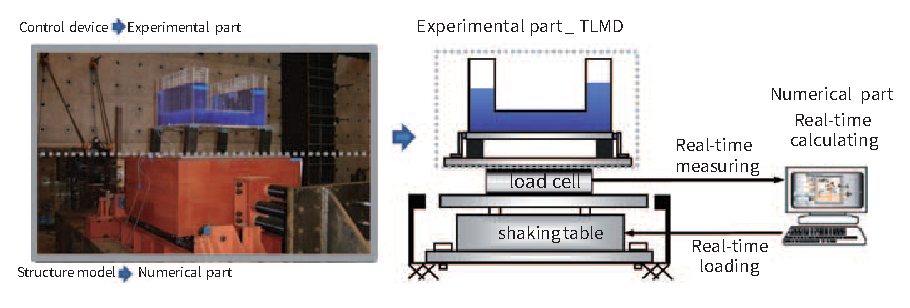
\includegraphics[width=0.8\textwidth] {figure/5-12.eps}
\caption{Conceptual view of the hybrid testing method of building with TLMD}
\label{fig:5-12}
\end{figure}




\subsubsection{Experimental setup}

The SDOF structure subjected to both the external and control forces is given by

\begin{equation}\label{eq:5-7}
m\ddot{x}+c\dot{x}+kx = F(t) - i(t)
\end{equation}

where $m$, $c$ and $k$ are the mass, damping coefficient and stiffness of the SDOF structure, respectively. $F(t)$ and $i(t)$ are the excitation force and TLMD control force measured at the load cell, respectively.

The state-space equation and the output equation for the absolute acceleration of the SDOF structural model such as Eq.~\eqref{eq:5-7} are represented by

\begin{align}
\dot{\matr{z}}&=\matr{A}\matr{z}+\matr{B}u \label{eq:5-8} \\
\bar{y_{1}}&=\matr{C}\matr{z} + \matr{D}u \label{eq:5-9}
\end{align}

where $z$ and $u$ are state variable and input vector, and can be expressed as $\matr{z}=\left[x, \dot{x}\right]^{\top}$ and $\matr{u} = \left[i(t), F(t)\right]^{\top}$, respectively. $\bar{y}_{1}$ is the absolute acceleration of the SDOF structural model, and the matrices $\matr{A}$, $\matr{B}$, $\matr{C}$ and $\matr{D}$ are follow-up as Eqs.~\eqref{eq:5-10}-\eqref{eq:5-13}, respectively.

\begin{align}
\matr{A}&=\begin{bmatrix} 0 & 1 \\ -k/m & -c/m \end{bmatrix} \label{eq:5-10} \\
\matr{B}&=\begin{bmatrix} 0 & 0 \\ -1/m & 1/m \end{bmatrix} \label{eq:5-11} \\
\matr{C}&=\begin{bmatrix} -k/m & -c/m \end{bmatrix} \label{eq:5-12} \\
\matr{D}&=\begin{bmatrix} -1/m & 1/m \end{bmatrix} \label{eq:5-13}
\end{align}

Finally, the controller both considering the numerical part of the SDOF structural model and the inverse transfer function of a shaking table is constructed to implement the hybrid testing method as shown in Figure~\ref{fig:5-16}. Figure~\ref{fig:5-17} shows the experimental configuration of the test. The hybrid testing method is fatal to the noise and phase error because the shaking table is vibrated by the numerical part which is calculated in real-time. Accordingly, the hybrid test using the Real-Time Window Target of the MATLAB Simulink with the sampling rate of 1000 Hz was implemented to minimize the calculation and phase error in the actual test. Figure~\ref{fig:5-18} is an excitation model of the Real-Time Window Target of the MATLAB Simulink, and it includes the inverse transfer function of the shaking table and numerical analysis of the SDOF structure.

\begin{figure}[ht]
\centering
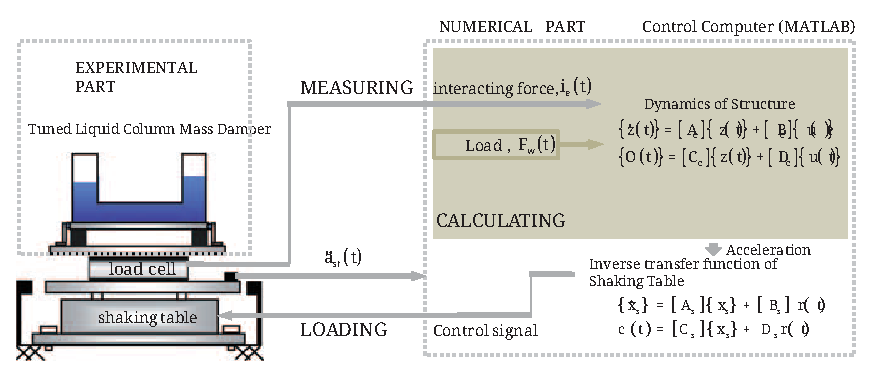
\includegraphics[width=0.8\textwidth] {figure/5-16.eps}
\caption{Design of the controller for the hybrid testing method}
\label{fig:5-16}
\end{figure}

\begin{figure}[ht]
\centering
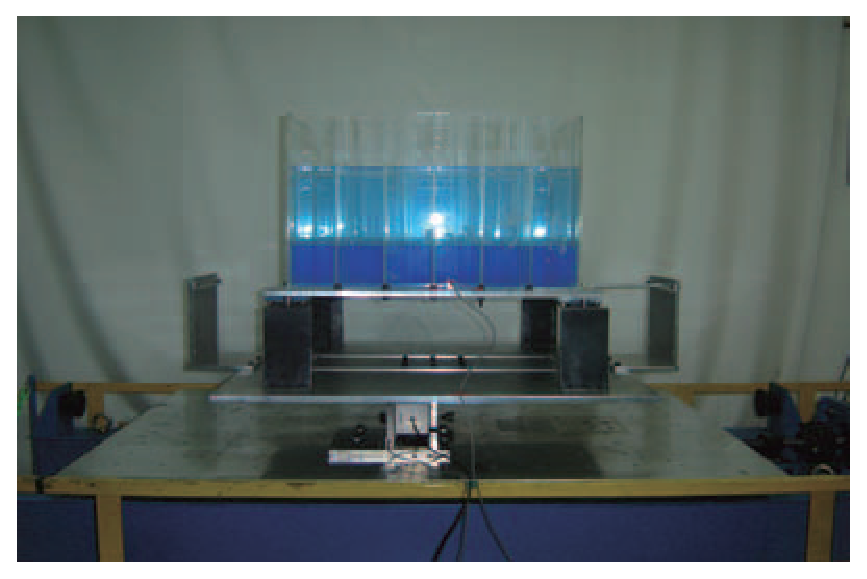
\includegraphics[width=0.8\textwidth] {figure/5-17.eps}
\caption{Photograph of the hybrid testing}
\label{fig:5-17}
\end{figure}

\begin{figure}[ht]
\centering
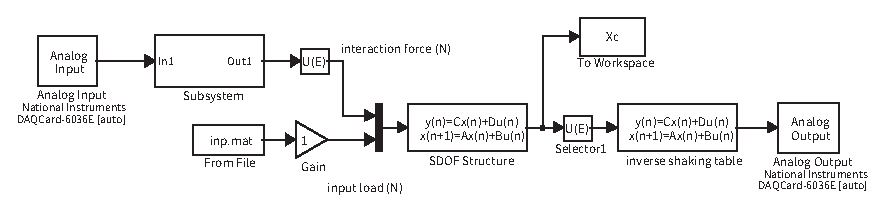
\includegraphics[width=0.8\textwidth] {figure/5-18.eps}
\caption{Design controller of the hybrid testing method (MATLAB Simulink Real-time Window Target)}
\label{fig:5-18}
\end{figure}








\clearpage

%\part{Experimantal Implementation}
\section{Experimental Verification}
\subsection{Experimental result of Substructuring technique}

The validity of the proposed substructuring technique as part of the hybrid testing method is verified for the experimental setting described in the previous sections. First, the shaking table test without feedback loop of accelerations measured from the experimental substructure into the shaking table controller in Figure~\ref{fig:2-11} is performed to confirm the validity of the proposed method experimentally. In this case, the third story acceleration of responses pre-calculated from the assumed whole building with structural parameters such as Eqs.~\eqref{eq:2-18} and \eqref{eq:2-19} is used as a reference signal in Figure~\ref{fig:2-8}. Figure~\ref{fig:2-12} compares the time histories and Fourier transform of the acceleration responses, which are measured from the experimental substructure and shaking table, with those calculated from the numerical analysis of the whole assumed structure. In other words, the responses corresponding to the 3rd, 4th and 5th story accelerations are compared. Also, Figures~\ref{fig:2-13}-\ref{fig:2-15} showing the variation of frequency components according to time lapse illustrate the spectrogram and contour plots of experimental and numerical accelerations of the 3rd, 4th and 5th story, respectively. As can be confirmed from Figure~\ref{fig:2-12}, the experimental accelerations obtained from the shaking table test without their feedback agree well with those obtained from the analysis of the whole assumed structure in both time and frequency domains. However, it can be observed that the small discrepancies are shown in the time histories of 4th and 5th story accelerations as shown from Figure~\ref{fig:2-12}, while the 3rd story acceleration is identical to the numerical one over the entire time history as known from Figures~\ref{fig:2-12}-\ref{fig:2-13}. These differences are caused by the inherent modes of experimental substructure; the frequency components of 2.5 and 8.6 Hz corresponding to the first and second modes of the experimental substructure, respectively, are observed in the measured acceleration of 4th story as known from Figure~\ref{fig:2-14}, and also the component of 2.5 Hz is expressed in the 5th story experimental acceleration as like Figure~\ref{fig:2-15}. It is considered that this tendency is especially conspicuous in the case of utilizing a lightly-damped testing model as an experimental substructure. Table 1 shows the frequency components observed in the time records of an experimental substructure from the test without its acceleration feedback and the natural frequencies calculated from the whole assumed structure with five stories. From Table~\ref{tab:2-1}, it can be noted that the first natural frequency of the experimental substructure is shifted from 2.5 Hz to 1.3 Hz by the dynamics of the three-story numerical substructure added to its base.
 Then, the substructuring testing expressed as Figure~\ref{fig:2-11} was carried out based on the acceleration feedback of the experimental substructure. Figure~\ref{fig:2-16} compares the responses measured by the test with the acceleration feedback of the experimental substructure with those calculated from the numerical analysis of the whole assumed structure with 5 DOFs. Also, Figures~\ref{fig:2-17}-\ref{fig:2-19} express the frequency components according to time lapse, which is observed in the measured responses from the test with feedback and the calculated ones of the 3rd, fourth and fifth story, respectively. As known from Figure~\ref{fig:2-16}, the inclination in entire time history responses measured from the proposed testing method agrees well with that calculated from the whole assumed structure. These are why the first mode responses of substructured system coincide well with those of the whole supposed system over the entire time range, as shown in Figures~\ref{fig:2-17}-\ref{fig:2-19}. However, as can be confirmed from Figures~\ref{fig:2-17}-\ref{fig:2-19}, instead of the second and third mode responses of the substructured system, those of the experimental substructure are observed from the testing results in the vicinity of 2.5 and 8.6 Hz. It is considered that in the process of the acceleration feedback of the experimental substructure, its fundamental modes affect to the numerical substructure and then the numerical error occurs in calculating the numerical substructure.

\begin{figure}[ht]
\centering
\subfigure[Time domain]{
   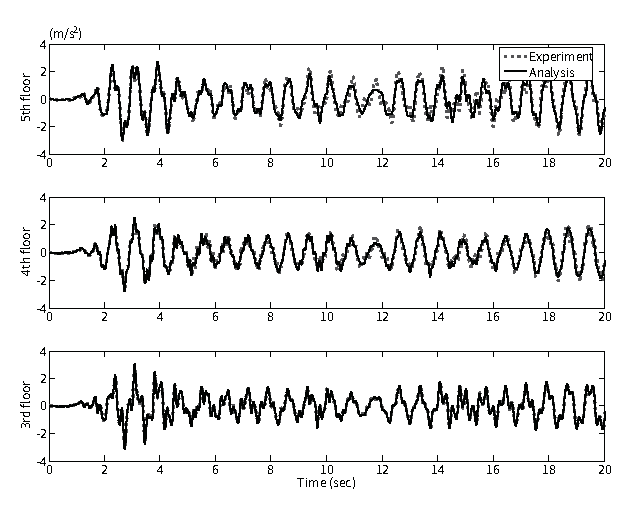
\includegraphics[width=0.8\textwidth] {figure/2-12a.eps}
   \label{fig:2-12a}
 }
 \subfigure[Frequency domain]{
   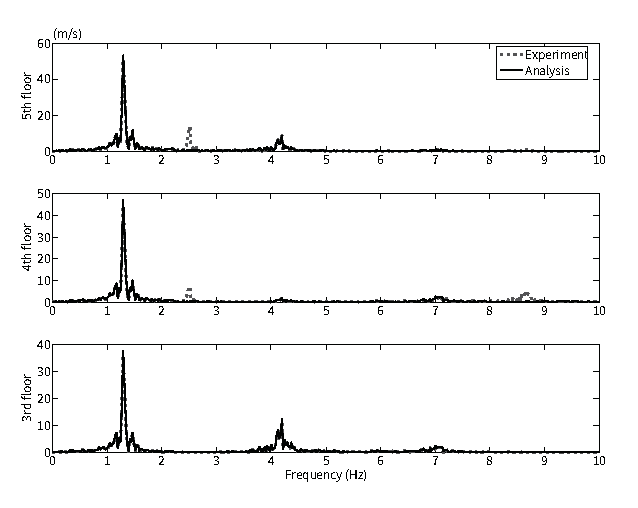
\includegraphics[width=0.8\textwidth] {figure/2-12b.eps}
   \label{fig:2-12b}
 }
\caption{Comparisons of results measured from the experiment without feedback and those calculated from numerical analysis.}
\label{fig:2-12}
\end{figure}

\begin{figure}[ht]
\centering
 \subfigure[Spectrogram of the response measured from the experiment without feedback]{
   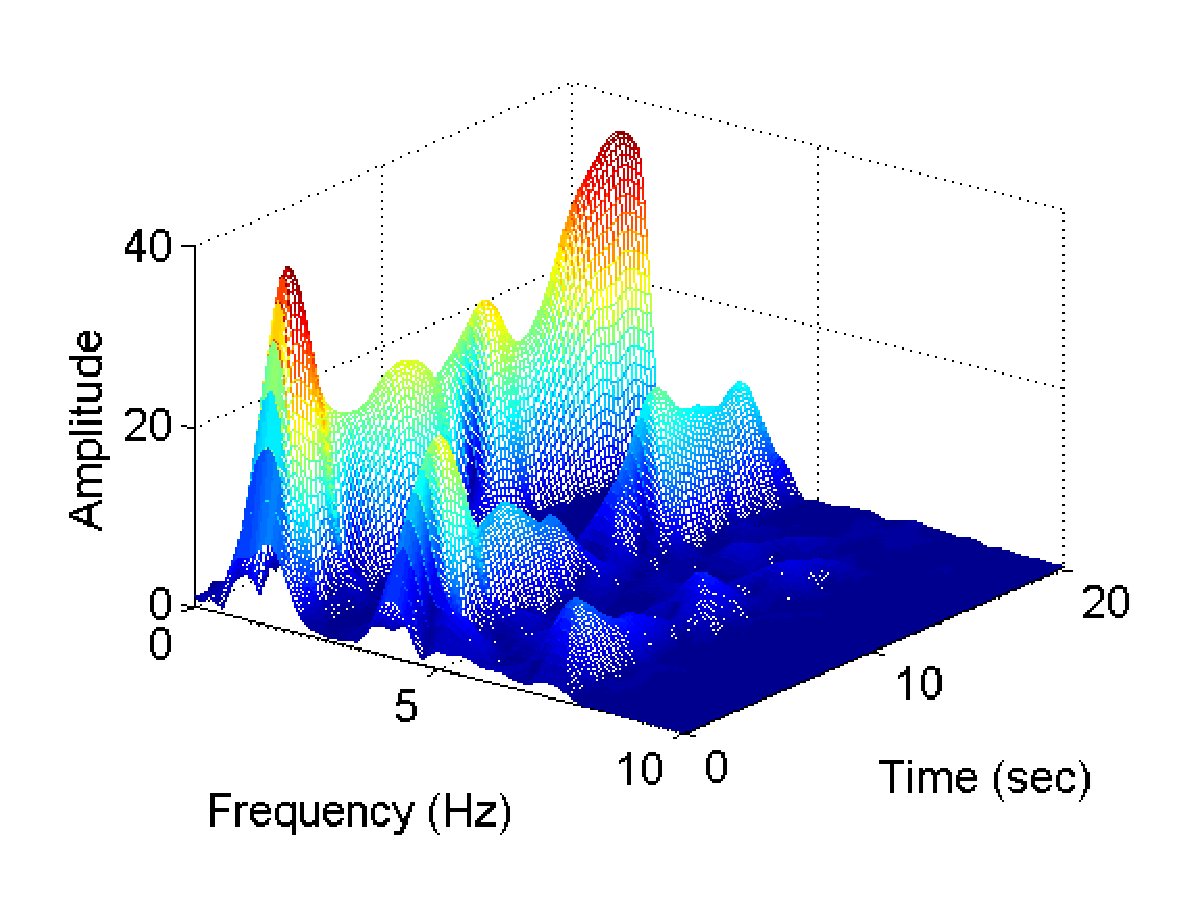
\includegraphics[width=0.45\textwidth] {figure/2-13a.eps}
   \label{fig:2-13a}
 }\hfill
 \subfigure[Spectrogram of the response calculated from the numerical analysis measured]{
   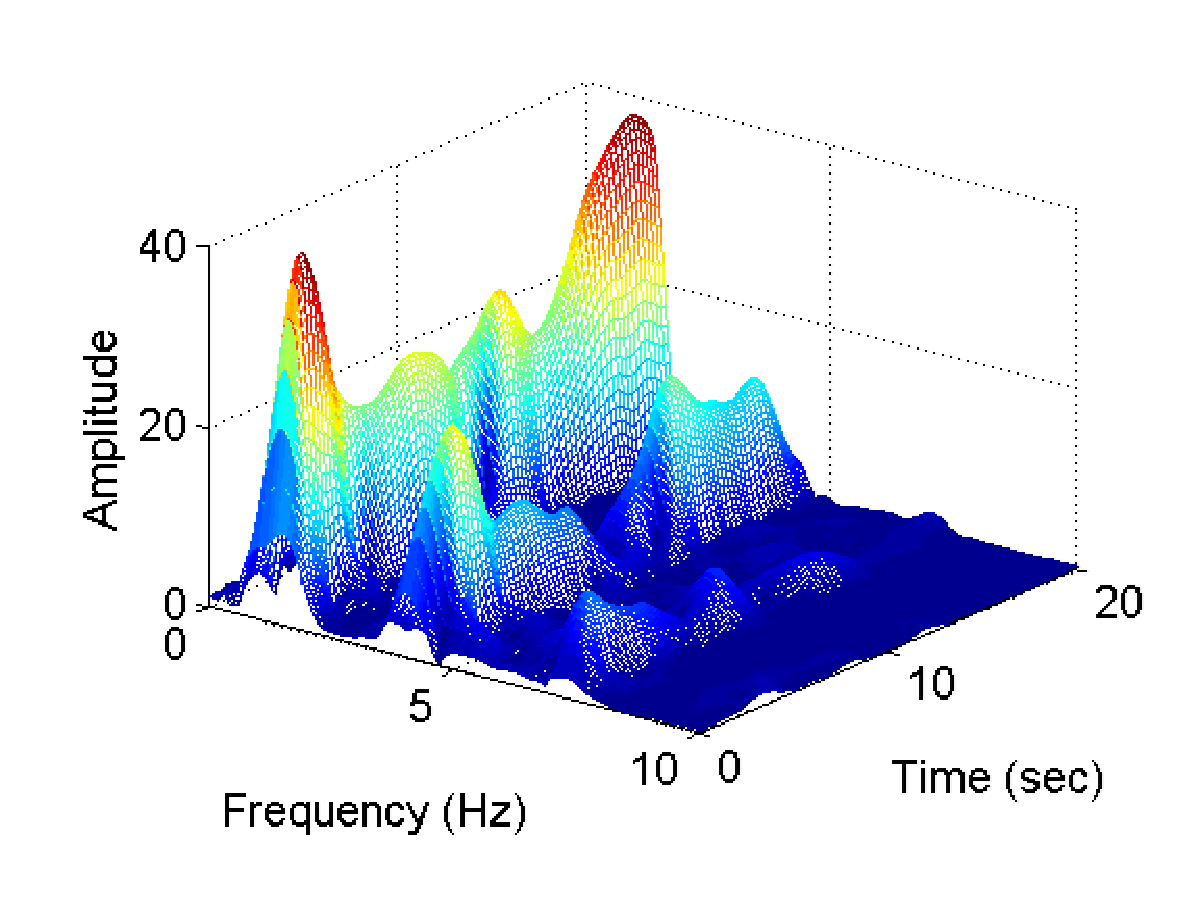
\includegraphics[width=0.45\textwidth] {figure/2-13b.eps}
   \label{fig:2-13b}
 }
 \subfigure[Contour plot of the response measured from the experiment without feedback]{
   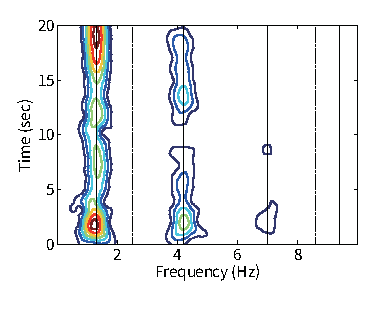
\includegraphics[width=0.45\textwidth] {figure/2-13c.eps}
   \label{fig:2-13c}
 }\hfill
 \subfigure[Contour plot of the response calculated from the numerical analysis measured]{
   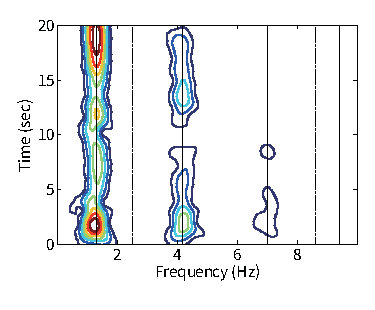
\includegraphics[width=0.45\textwidth] {figure/2-13d.eps}
   \label{fig:2-13d}
 }
\caption{Spectrograms and contour plots of the 3rd story acceleration measured from the experiment without feedback and that calculated from the numerical analysis.}
\label{fig:2-13}
\end{figure}

\begin{figure}[ht]
\centering
 \subfigure[Spectrogram of the response measured from the experiment without feedback]{
   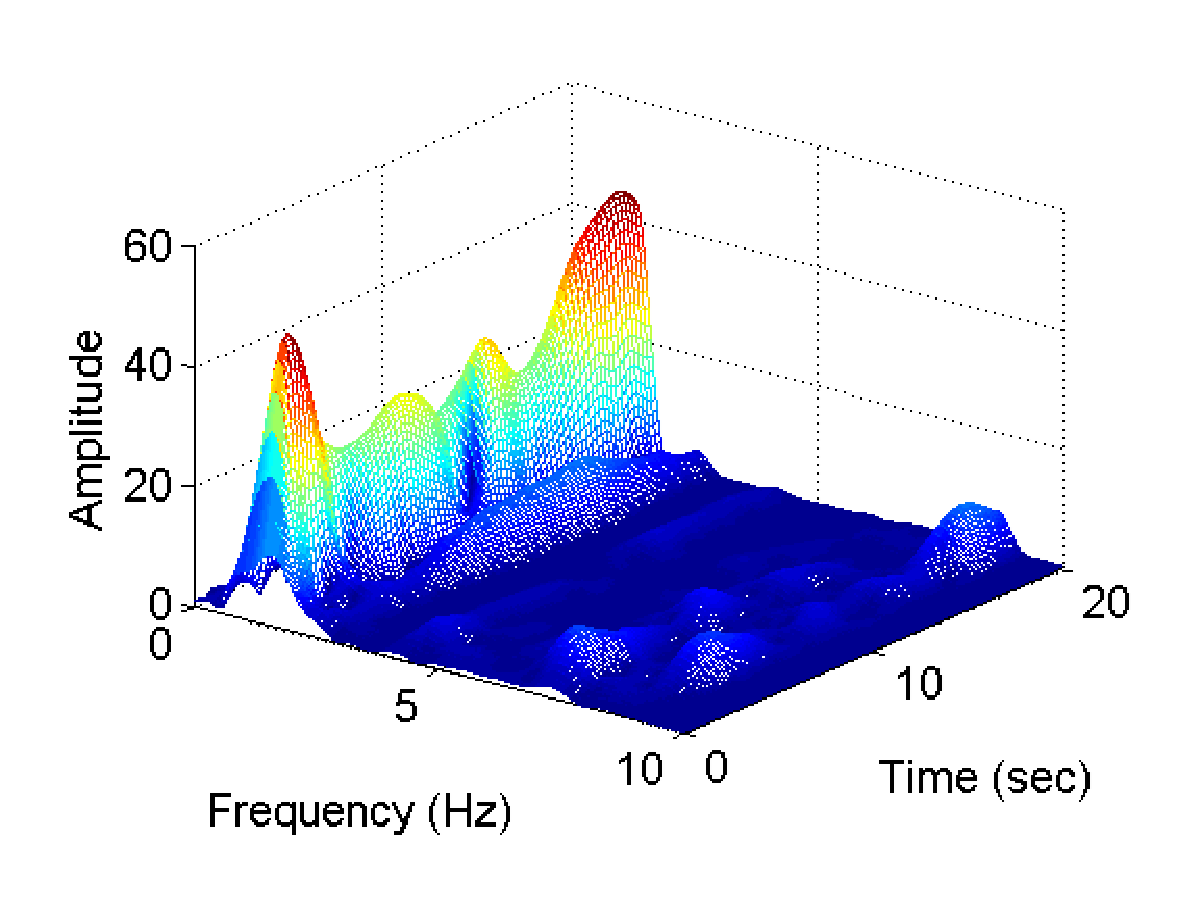
\includegraphics[width=0.45\textwidth] {figure/2-14a.eps}
   \label{fig:2-14a}
 }\hfill
 \subfigure[Spectrogram of the response calculated from the numerical analysis measured]{
   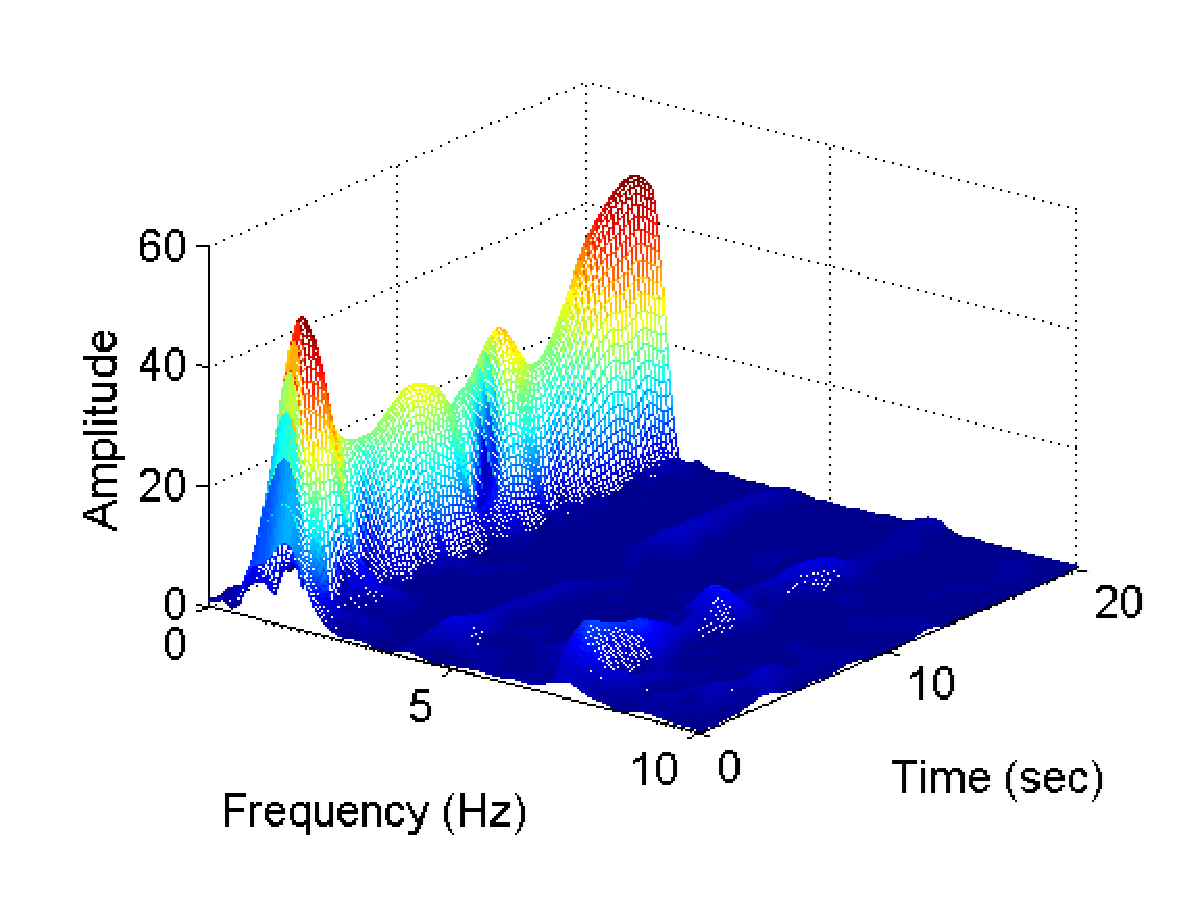
\includegraphics[width=0.45\textwidth] {figure/2-14b.eps}
   \label{fig:2-14b}
 }
 \subfigure[Contour plot of the response measured from the experiment without feedback]{
   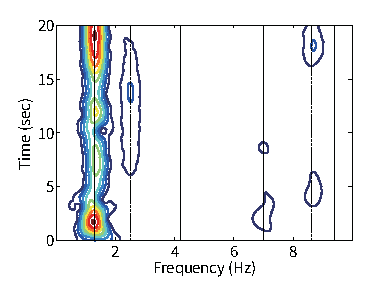
\includegraphics[width=0.45\textwidth] {figure/2-14c.eps}
   \label{fig:2-14c}
 }\hfill
 \subfigure[Contour plot of the response calculated from the numerical analysis measured]{
   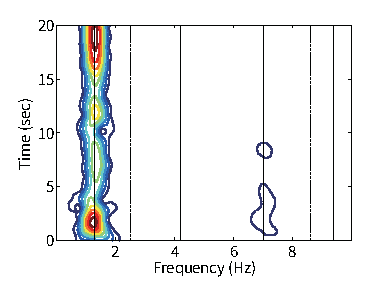
\includegraphics[width=0.45\textwidth] {figure/2-14d.eps}
   \label{fig:2-14d}
 }
\caption{Spectrograms and contour plots of the 4th story acceleration measured from the experiment without feedback and that calculated from the numerical analysis.}
\label{fig:2-14}
\end{figure}

\begin{figure}[ht]
\centering
 \subfigure[Spectrogram of the response measured from the experiment without feedback]{
   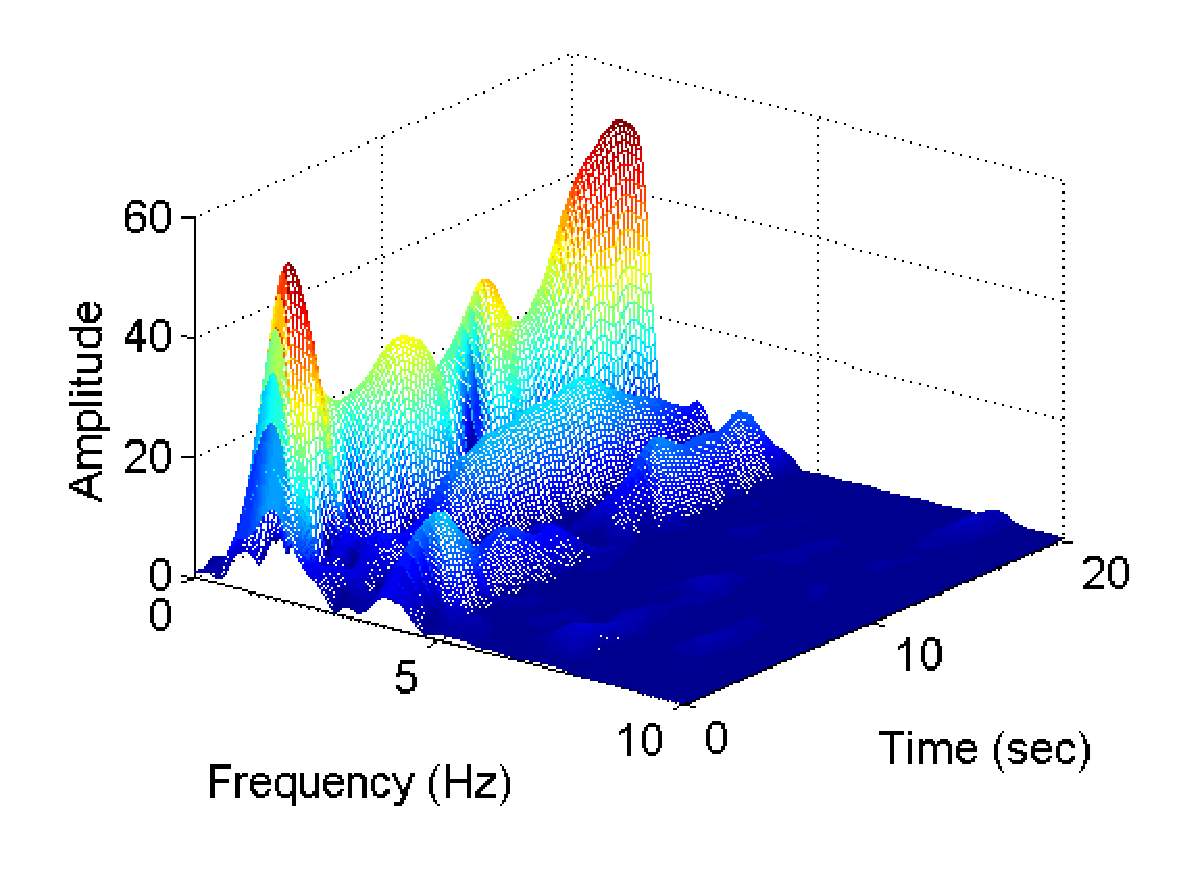
\includegraphics[width=0.45\textwidth] {figure/2-15a.eps}
   \label{fig:2-15a}
 }\hfill
 \subfigure[Spectrogram of the response calculated from the numerical analysis measured]{
   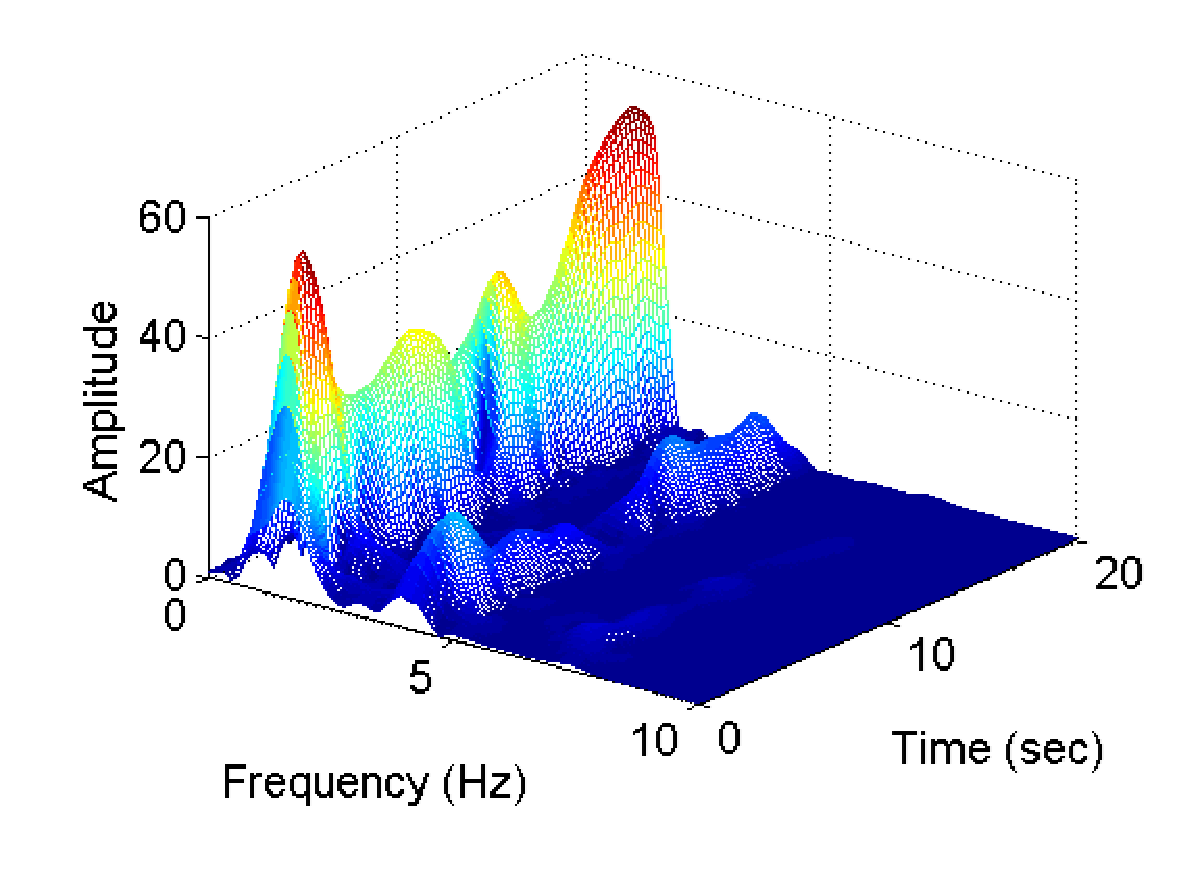
\includegraphics[width=0.45\textwidth] {figure/2-15b.eps}
   \label{fig:2-15b}
 }
 \subfigure[Contour plot of the response measured from the experiment without feedback]{
   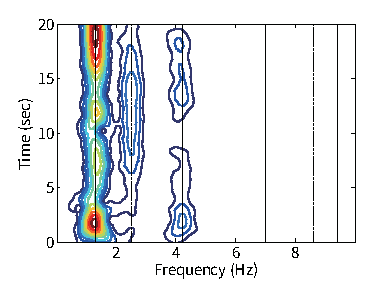
\includegraphics[width=0.45\textwidth] {figure/2-15c.eps}
   \label{fig:2-15c}
 }\hfill
 \subfigure[Contour plot of the response calculated from the numerical analysis measured]{
   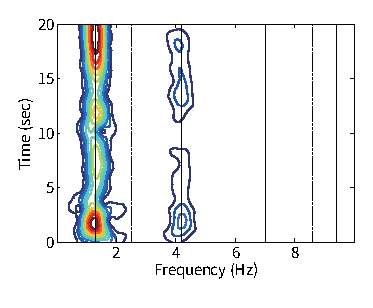
\includegraphics[width=0.45\textwidth] {figure/2-15d.eps}
   \label{fig:2-15d}
 }
\caption{Spectrograms and contour plots of the 5th story acceleration measured from the experiment without feedback and that calculated from the numerical analysis.}
\label{fig:2-15}
\end{figure}

\begin{figure}[ht]
\centering
\subfigure[Time domain]{
   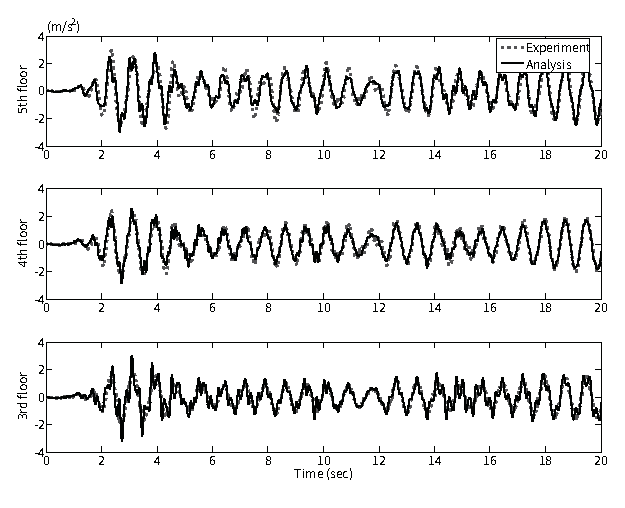
\includegraphics[width=0.8\textwidth] {figure/2-16a.eps}
   \label{fig:2-16a}
 }
 \subfigure[Frequency domain]{
   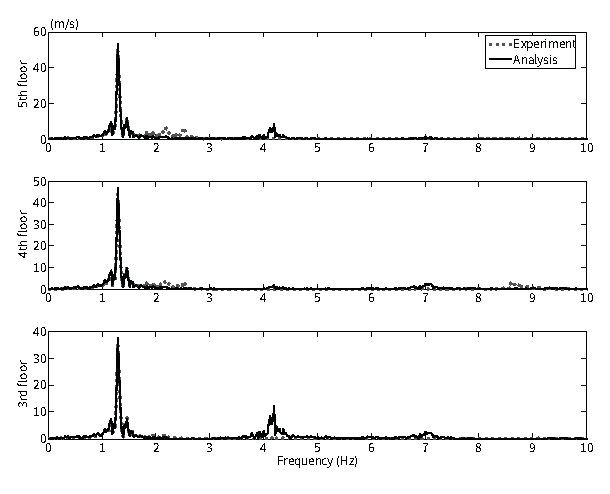
\includegraphics[width=0.8\textwidth] {figure/2-16b.eps}
   \label{fig:2-16b}
 }
\caption{Comparisons between results from the experiment with feedback and those from analysis.}
\label{fig:2-16}
\end{figure}

\begin{figure}[ht]
\centering
 \subfigure[Spectrogram of the response measured from the experiment without feedback]{
   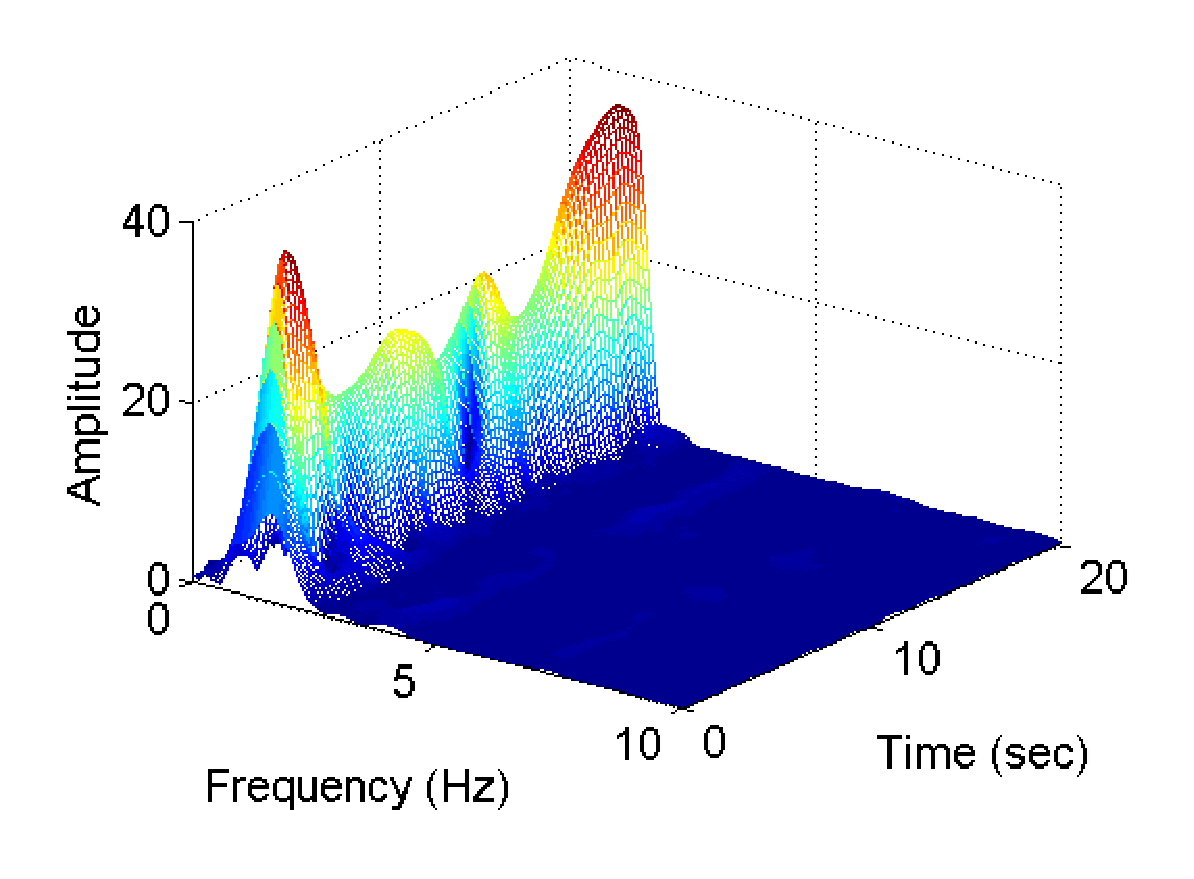
\includegraphics[width=0.45\textwidth] {figure/2-17a.eps}
   \label{fig:2-17a}
 }\hfill
 \subfigure[Spectrogram of the response calculated from the numerical analysis measured]{
   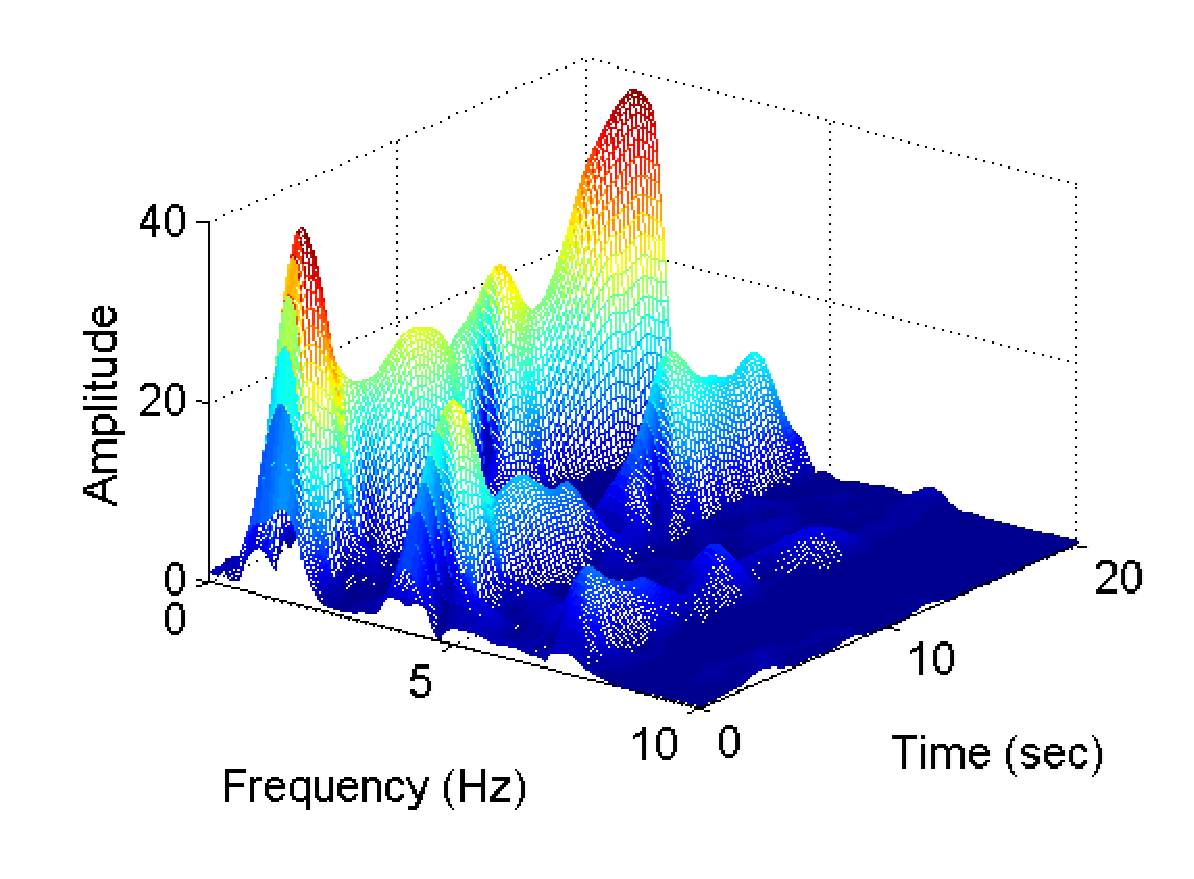
\includegraphics[width=0.45\textwidth] {figure/2-17b.eps}
   \label{fig:2-17b}
 }
 \subfigure[Contour plot of the response measured from the experiment without feedback]{
   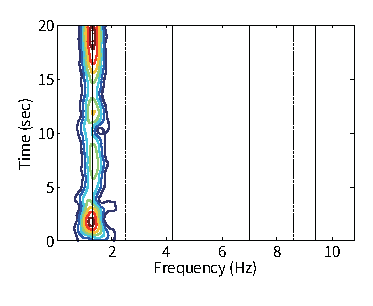
\includegraphics[width=0.45\textwidth] {figure/2-17c.eps}
   \label{fig:2-17c}
 }\hfill
 \subfigure[Contour plot of the response calculated from the numerical analysis measured]{
   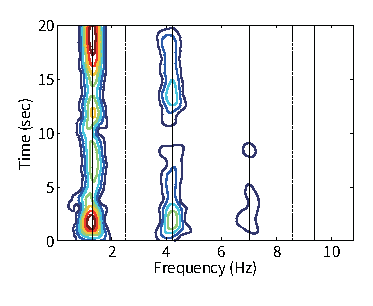
\includegraphics[width=0.45\textwidth] {figure/2-17d.eps}
   \label{fig:2-17d}
 }
\caption{Spectrograms and contour plots of the 3rd story acceleration measured from the experiment with feedback and that calculated from the numerical analysis.}
\label{fig:2-17}
\end{figure}

\begin{figure}[ht]
\centering
 \subfigure[Spectrogram of the response measured from the experiment without feedback]{
   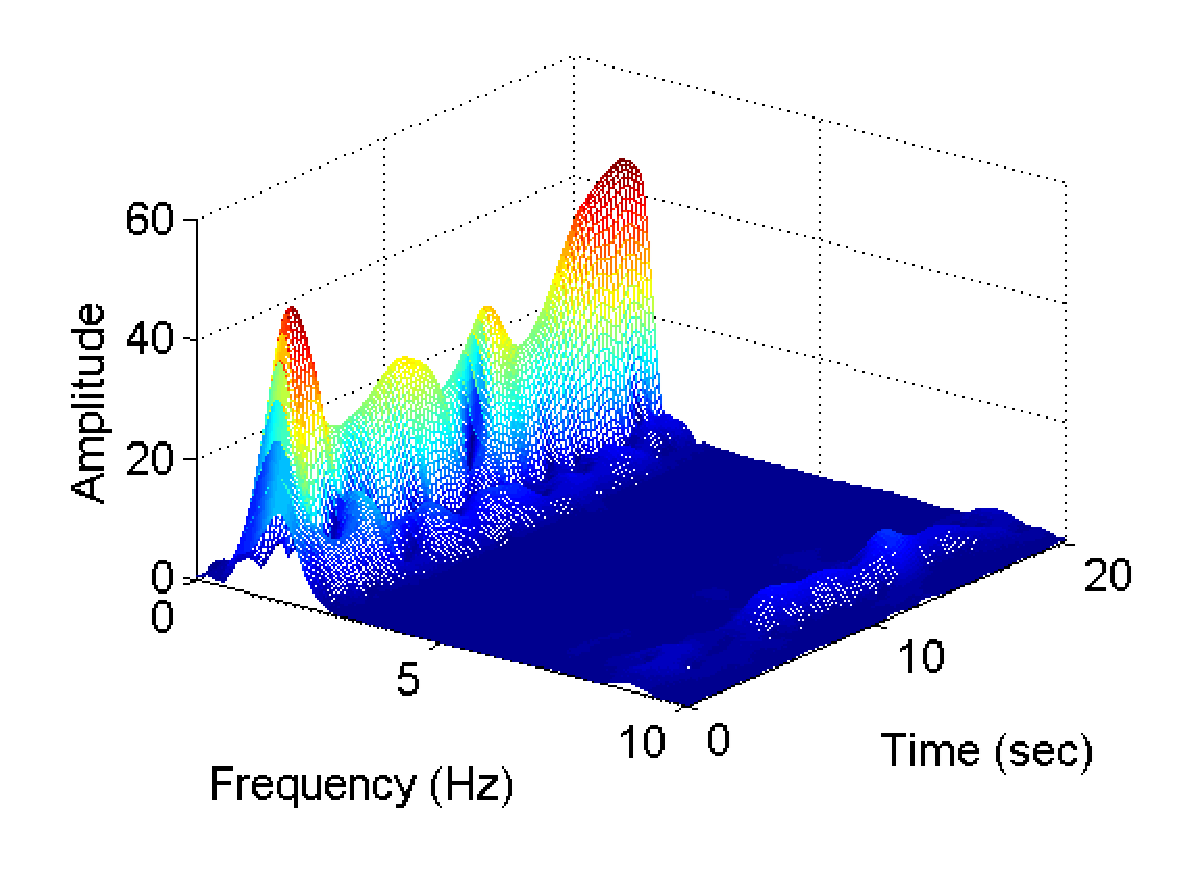
\includegraphics[width=0.45\textwidth] {figure/2-18a.eps}
   \label{fig:2-18a}
 }\hfill
 \subfigure[Spectrogram of the response calculated from the numerical analysis measured]{
   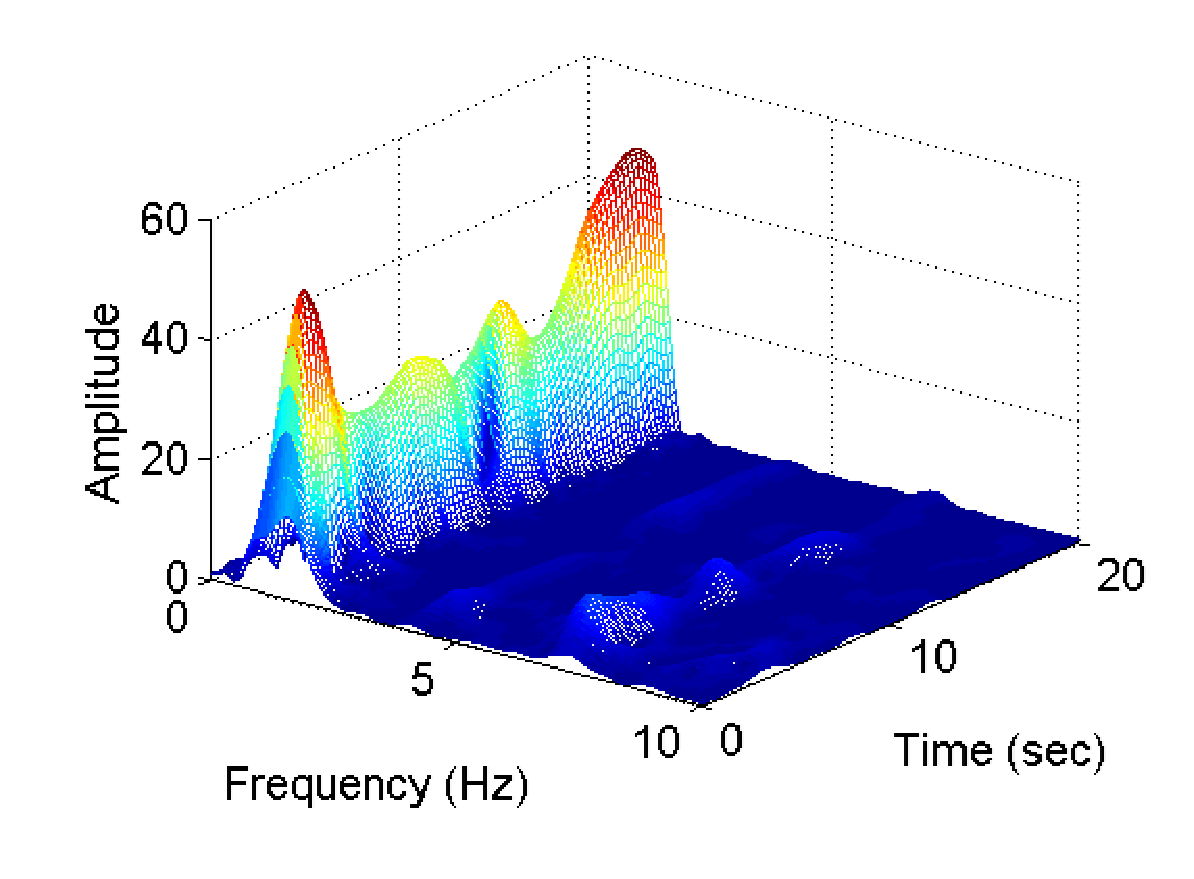
\includegraphics[width=0.45\textwidth] {figure/2-18b.eps}
   \label{fig:2-18b}
 }
 \subfigure[Contour plot of the response measured from the experiment without feedback]{
   \includegraphics[width=0.45\textwidth] {figure/2-18c.eps}
   \label{fig:2-18c}
 }\hfill
 \subfigure[Contour plot of the response calculated from the numerical analysis measured]{
   \includegraphics[width=0.45\textwidth] {figure/2-18d.eps}
   \label{fig:2-18d}
 }
\caption{Spectrograms and contour plots of the 4th story acceleration measured from the experiment with feedback and that calculated from the numerical analysis.}
\label{fig:2-18}
\end{figure}

\begin{figure}[ht]
\centering
 \subfigure[Spectrogram of the response measured from the experiment without feedback]{
   \includegraphics[width=0.45\textwidth] {figure/2-19a.eps}
   \label{fig:2-19a}
 }\hfill
 \subfigure[Spectrogram of the response calculated from the numerical analysis measured]{
   \includegraphics[width=0.45\textwidth] {figure/2-19b.eps}
   \label{fig:2-19b}
 }
 \subfigure[Contour plot of the response measured from the experiment without feedback]{
   \includegraphics[width=0.45\textwidth] {figure/2-19c.eps}
   \label{fig:2-19c}
 }\hfill
 \subfigure[Contour plot of the response calculated from the numerical analysis measured]{
   \includegraphics[width=0.45\textwidth] {figure/2-19d.eps}
   \label{fig:2-19d}
 }
\caption{Spectrograms and contour plots of the 5th story acceleration measured from the experiment with feedback and that calculated from the numerical analysis.}
\label{fig:2-19}
\end{figure}

% \clearpage
% \section{Concluding Remarks}
% In this study, a new real-time substructuring technique for the shaking table test was proposed. The proposed substructuring technique adopts the upper part of the whole structure as the experimental substructure, which corresponds to a physical test model. In order to verify the validity and accuracy of the proposed technique, a shaking table test was conducted. The result of the study can be summarized as follows.
% \begin{enumerate}
% \item To reduce the distortion of the interface acceleration, the inverse transfer function of the shaking table was identified, and its state space realization was implemented in the shaking table controller.
% \item In this paper, the linear transfer function approach for controlling the motion of a shaking table was considered to verify the proposed method for a linear experimental part experimentally. However, this approach would be inappropriate in a coupled non-linear system leading to experimental instability. Therefore, in such case the controller using the inverse transfer function of shaking table, shown in Fig. 11, would be modified to compensate an experimental instability.
% \item The interface force between the experimental and numerical substructures was obtained using only acceleration measurement and mass information so that high-capacity loads cell and installation jigs are not required in the experiment. 
% \item The proposed method basing the interface force measurement on acceleration measurements from an experimental substructure is partially available only when the mass distribution is discrete - for example this would be applicable to the TMD as an experimental part. Also, the interface force measurement using force transducers is required to perform the proposed method when wind forces are applied to the experimental substructure.
% \item Experimental results demonstrate that the proposed real-time substructuring technique can reproduce the dynamic behavior of the whole assumed structure.
% \item Unexpected vibration of the experimental substructure can be induced by the feedback of responses including its inherent natural modes and then by the error occurred in calculating the numerical substructure.
% \item It is considered that to minimize the effect of natural modes of an experimental substructure on the substructured system, the structural model as heavily-damped as possible would be used as an experimental part.
% \item The proposed technique can be extended to the real-time substructuring technique with the middle part of a whole structure in combination with the conventional substructuring technique employing lower part as the experimental substructure.
% \end{enumerate}


\clearpage
\subsection{Hybrid Testing Method of a Single Story Strcuture with a TLD}
In this section, experimental verification of the hybrid testing method is conducted for a single story steel frame with a TLD. First, the conventional TLD-structure interaction model shown in Figure~\ref{fig:3-4a} is tested. Then, the hybrid testing method shown in Figure~\ref{fig:3-4b}, which incorporates the single story steel frame in the numerical calculation, is performed and the results from the two testing methods are compared to each other.
For the numerical structural model used in the hybrid testing method, the single story steel frame is assumed to be an SDOF mass-damping-spring system. The structure has $0.6m$ of width, $1.0m$ of height and $169.7kg$ of measured floor mass. El Centro, Hachinohe, Mexico City, and Northridge earthquake waves were realized by the shaking table, and the resulting absolute accelerations of the floor and the shaking table were measured. The system identification was conducted using the measured absolute accelerations. The identified parameters slightly vary according to input earthquake waves. The averaged damping and stiffness coefficients are 14.6$N\cdot s/m$ and $9914.3N/m$, respectively, which correspond to $1.23Hz$ of structural natural frequency. The TLD shown in Figure~\ref{fig:3-4} has the size of $31(cm)\times14(cm)\times20(cm)$. The level of water in the TLD was adjusted to have $3.4cm$ that is theoretically calculated based on the linear wave theory\citep{soong1997passive} for the TLD to have fundamental sloshing frequency tuned to the identified structural natural frequency. As a result, the mass ratio of the TLD to the structure is about $1.3\%$. To confirm whether the numerically calculated frequency of the TLD is modulated to the structural one, the transfer function is shown in Figure~\ref{fig:3-5}, from the shaking table acceleration to the shear force by the TLD, was obtained by using the white noise excitation. It is observed in Figure~\ref{fig:3-5} that the TLD has the sloshing frequency of $1.25Hz$ which is very close to the structural natural frequency of $1.23Hz$.

\begin{figure}[!ht]
\centering
\subfigure[Conventional shaking table test]{
   \includegraphics[width=0.8\textwidth] {figure/3-4a.eps}
   \label{fig:3-4a}
 }
 \subfigure[Hybrid shaking table test]{
   \includegraphics[width=0.8\textwidth] {figure/3-4b.eps}
   \label{fig:3-4b}
 }
\caption{TLD-structure interaction experimental system.}
\label{fig:3-4}
\end{figure}

\begin{figure}[!ht]
\centering
\includegraphics[width=0.8\textwidth] {figure/3-5.eps}
\caption{TLD transfer function from the table acceleration to the base shear force}
\label{fig:3-5}
\end{figure}

At first, the conventional shaking table test is shown in Figure~\ref{fig:3-4a} is performed to investigate the seismic response control performance of the TLD. Previously mentioned four earthquake records are scaled to have the peak acceleration of 100 gals and used to excite the TLD-structure system. Figures~\ref{fig:3-6} and \ref{fig:3-7} show the measured structural acceleration responses in the time and frequency domains, respectively. It is observed from Figure~\ref{fig:3-6} that acceleration in the latter part of the whole response history is significantly reduced. This phenomenon is a common tendency in the structural response controlled by a tuned mass-type control device since it makes an effect when the structural response is governed by the fundamental mode after initial high impulse like component has passed. In response to Mexico-city earthquake excitation, as shown in Figure~\ref{fig:3-7c}, the first peak corresponding to the major frequency component of the earthquake itself is not controlled, but the response in the region of the TLD modulation frequency is reduced to nearly zero.

\begin{figure}[!ht]
\centering
 \subfigure[El Centro earthquake]{
   \includegraphics[width=0.8\textwidth] {figure/3-6a.eps}
   \label{fig:3-6a}
 }
 \subfigure[Hachinohe earthquake]{
   \includegraphics[width=0.8\textwidth] {figure/3-6b.eps}
   \label{fig:3-6b}
 }
 \subfigure[Mexico city earthquake]{
   \includegraphics[width=0.8\textwidth] {figure/3-6c.eps}
   \label{fig:3-6c}
 }
 \subfigure[Northridge earthquake]{
   \includegraphics[width=0.8\textwidth] {figure/3-6d.eps}
   \label{fig:3-6d}
 }
\caption{Structural acceleration in the time domain measured from the conventional shaking table test of TLD-structure interaction system (dotted line : without control, solid line : with control)}
\label{fig:3-6}
\end{figure}

\begin{figure}[!ht]
\centering
 \subfigure[El Centro earthquake]{
   \includegraphics[width=0.45\textwidth] {figure/3-7a.eps}
   \label{fig:3-7a}
 }\hfill
 \subfigure[Hachinohe earthquake]{
   \includegraphics[width=0.45\textwidth] {figure/3-7b.eps}
   \label{fig:3-7b}
 }
 \subfigure[Mexico city earthquake]{
   \includegraphics[width=0.45\textwidth] {figure/3-7c.eps}
   \label{fig:3-7c}
 }\hfill
 \subfigure[Northridge earthquake]{
   \includegraphics[width=0.45\textwidth] {figure/3-7d.eps}
   \label{fig:3-7d}
 }
\caption{Structural acceleration in the frequency domain measured from the conventional shaking table test of TLD-structure interaction system (dotted line : without control, solid line : with control)}
\label{fig:3-7}
\end{figure}

Then, the hybrid testing method is applied with the experimental set-up shown in Figure~\ref{fig:3-4b}. For its implementation for the controlled case, the identified structural parameters are reflected in the numerical part expressed by the shaded region in the integrated controller shown in Figure~\ref{fig:3-3}. The continuous filters are converted into discrete ones with a time interval of 0.01 second. Figures~\ref{fig:3-8} and \ref{fig:3-9} compare the controlled accelerations obtained by performing the conventional and the hybrid testing method in time and frequency domains, respectively. The effectiveness of the hybrid testing method is verified by the fact that the experimental results from two methods coincide well with each other on the whole. The small discrepancies existing in the controlled responses subjected to El Centro and Hachinohe earthquakes are considered to result from the underestimation of damping coefficients in the numerical structural model since averaged parameters for the four earthquake data were used.

\begin{figure}[!ht]
\centering
 \subfigure[El Centro earthquake]{
   \includegraphics[width=0.8\textwidth] {figure/3-8a.eps}
   \label{fig:3-8a}
 }
 \subfigure[Hachinohe earthquake]{
   \includegraphics[width=0.8\textwidth] {figure/3-8b.eps}
   \label{fig:3-8b}
 }
 \subfigure[Mexico city earthquake]{
   \includegraphics[width=0.8\textwidth] {figure/3-8c.eps}
   \label{fig:3-8c}
 }
 \subfigure[Northridge earthquake]{
   \includegraphics[width=0.8\textwidth] {figure/3-8d.eps}
   \label{fig:3-8d}
 }
\caption{Comparisons of controlled structural accelerations in the time domain
(dotted line : conventional shaking table test, solid line : hybrid shaking table test)
}
\label{fig:3-8}
\end{figure}

\begin{figure}[!ht]
\centering
 \subfigure[El Centro earthquake]{
   \includegraphics[width=0.45\textwidth] {figure/3-9a.eps}
   \label{fig:3-9a}
 }\hfill
 \subfigure[Hachinohe earthquake]{
   \includegraphics[width=0.45\textwidth] {figure/3-9b.eps}
   \label{fig:3-9b}
 }
 \subfigure[Mexico city earthquake]{
   \includegraphics[width=0.45\textwidth] {figure/3-9c.eps}
   \label{fig:3-9c}
 }\hfill
 \subfigure[Northridge earthquake]{
   \includegraphics[width=0.45\textwidth] {figure/3-9d.eps}
   \label{fig:3-9d}
 }
\caption{Comparisons of controlled structural accelerations in the frequency domain (dotted line : conventional shaking table test, solid line : hybrid shaking table test)}
\label{fig:3-9}
\end{figure}

\clearpage
\subsection{Hybrid Testing Method of Three Story Structure with a TLD}
The control performance of a TLD installed in a three-story structure is investigated by using the hybrid testing method. The structure is assumed to be a three story shear-type model, which has identical story properties as follows; $m_{i}=128.8kg$, $c_{i}=13.52N\cdot s/m$, $k_{i}=33908N/m$ for $i=1,2,3$. The structure has natural frequencies of $1.15Hz$, $3.22Hz$ and $4.65Hz$. The TLD discussed in the previous section is used, and its water level is modulated to $4.6cm$ for the TLD to have sloshing frequency of $1.15Hz$. As a result, the mass ratio of the TLD to the structure is about $2\%$. The four earthquake waves used for the excitation of the single story steel frame were scaled to have peak acceleration of $40gal$. The uncontrolled structural responses were obtained by removing the feedback loop of the TLD-generated interacting force, which causes the numerical structural model to be excited only by the base earthquake motion. 
Figures~\ref{fig:3-10} and \ref{fig:3-11} compare the uncontrolled and controlled accelerations of the third story in time and frequency domains, respectively, which is realized by the shaking table through the hybrid testing method. It is observed that the structural accelerations are significantly reduced by the TLD, especially in the region of the fundamental frequency. Table~\ref{tab:3-1} indicates that the acceleration is reduced by $4-30\%$ in peak and by $18-60\%$ in RMS responses. It is also identified in Figure~\ref{fig:3-11d} that the TLD lessens the additional second mode response of the structure. Figure~\ref{fig:3-12} shows the typical sloshing and slamming behaviors of the water in the TLD tanks during the experiment, which occur in the small and large amplitude of the water motion, respectively\citep{yalla2001liquid}.

\begin{figure}[!ht]
\centering
 \subfigure[El Centro earthquake]{
   \includegraphics[width=0.8\textwidth] {figure/3-10a.eps}
   \label{fig:3-10a}
 }
 \subfigure[Hachinohe earthquake]{
   \includegraphics[width=0.8\textwidth] {figure/3-10b.eps}
   \label{fig:3-10b}
 }
 \subfigure[Mexico city earthquake]{
   \includegraphics[width=0.8\textwidth] {figure/3-10c.eps}
   \label{fig:3-10c}
 }
 \subfigure[Northridge earthquake]{
   \includegraphics[width=0.8\textwidth] {figure/3-10d.eps}
   \label{fig:3-10d}
 }
\caption{Absolute accelerations in the time domain, measured from the top story of MDOF structure with a TLD by the hybrid testing method (dotted line : without control, solid line : with control))
}
\label{fig:3-10}
\end{figure}

\begin{figure}[!ht]
\centering
 \subfigure[El Centro earthquake]{
   \includegraphics[width=0.45\textwidth] {figure/3-11a.eps}
   \label{fig:3-11a}
 }\hfill
 \subfigure[Hachinohe earthquake]{
   \includegraphics[width=0.45\textwidth] {figure/3-11b.eps}
   \label{fig:3-11b}
 }
 \subfigure[Mexico city earthquake]{
   \includegraphics[width=0.45\textwidth] {figure/3-11c.eps}
   \label{fig:3-11c}
 }\hfill
 \subfigure[Northridge earthquake]{
   \includegraphics[width=0.45\textwidth] {figure/3-11d.eps}
   \label{fig:3-11d}
 }
\caption{Absolute accelerations in the frequency domain, measured from the top story of MDOF structure with a TLD by the hybrid testing method (dotted line : without control, solid line : with control)}
\label{fig:3-11}
\end{figure}

\begin{figure}[!ht]
\centering
 \subfigure[Sloshing of TLD]{
   \includegraphics[width=0.45\textwidth] {figure/3-12a.eps}
   \label{fig:3-12a}
 }\hfill
 \subfigure[Slamming of TLD]{
   \includegraphics[width=0.45\textwidth] {figure/3-12b.eps}
   \label{fig:3-12b}
 }
\caption{Behaviors of a TLD under the earthquake motion}
\label{fig:3-12}
\end{figure}

\begin{table}[ht]
\centering
\begin{tabularx}{\textwidth}{b|s|s|s|s}
\toprule[1pt]\midrule[0.3pt]
Responses$(g)$&El Centro&Hachinohe&Mexico City&Northridge\\ \midrule[0.3pt]
\textit{Peak acceleration}&&&&\\
Uncontrolled& 3.85&2.71&2.63&1.34\\
Controlled& 2.69&2.19&252&1.34\\
\textit{RMS acceleration}&&&&\\
Uncontrolled&1.91&1.36&0.54&0.33\\
Controlled&0.74&0.66&0.45&0.27\\ \bottomrule
\end{tabularx}
\caption{Uncontrolled and controlled responses of a combined TLD–MDOF structure system}
\label{tab:3-1}
\end{table}

% \section{Concluding Remarks}
% In this study, a real-time hybrid shaking table test was conducted to verify the seismic control performance of the TLD installed in the building structures. The TLD installed at the top floor of the structure is physically tested, and simultaneously numerical calculation is carried out for the assumed analytical structural model. Comparison between the structural responses obtained by the hybrid testing method and the conventional shaking table test of a single story steel frame with TLD indicates that the performance of the TLD can be accurately evaluated using the hybrid testing method without the physical structural model. Finally, the uncontrolled and TLD-controlled structural responses of a three-story structure are obtained by the hybrid testing method in both time, and frequency domains, showing that TLD can effectively mitigate the seismic responses of building structures and the hybrid testing method can reproduce the dynamic behavior of TLD-structure interaction systems for both the uncontrolled and controlled case. The hybrid testing method can also be applied to the performance evaluation of tuned liquid column damper which has strong inherent nonlinearity.








\subsection{Hybrid Testing Method of a Single Story Structure with a TLCD}
At first, the conventional shaking table test with this TLCD shown in Figure~\ref{fig:4-4a} is performed to reduce the structural response. Two earthquake records with the maximum acceleration of $100gal$ due to the shaking table performance are used to excite the TLCD-structure system with control case. Then, the hybrid shaking table test is conducted with the experimental set-up shown in Figure~\ref{fig:4-4b}. For its experimental implementation, the identified structural parameters are reflected in the numerical part expressed by the shaded region in the integrated controller shown in Figure~\ref{fig:4-3}. The continuous filters in the figure are converted into discrete ones with a time step of 0.01 sec in the actual implementation of the experiment. Figure~\ref{fig:4-5} compare the controlled accelerations experimentally measured by implementing the conventional and the hybrid testing method in both time and frequency domain, respectively. The validity of the hybrid testing method performed in this paper is verified from the fact that the experimental results from two methods well coincide with each other on the whole.

\begin{figure}[!ht]
\centering
 \subfigure[El Centro Earthquake(time domain)]{
   \includegraphics[width=0.45\textwidth] {figure/4-5a.eps}
   \label{fig:4-5a}
 }\hfill
 \subfigure[El Centro Earthquake(frequency domain)]{
   \includegraphics[width=0.45\textwidth] {figure/4-5b.eps}
   \label{fig:4-5b}
 }
 \subfigure[Kobe Earthquake(time domain)]{
   \includegraphics[width=0.45\textwidth] {figure/4-5c.eps}
   \label{fig:4-5c}
 }\hfill
 \subfigure[Kobe Earthquake(frequency domain)]{
   \includegraphics[width=0.45\textwidth] {figure/4-5d.eps}
   \label{fig:4-5d}
 }
\caption{Comparisons between the results from the conventional testing method(dotted line) and those from the hybrid testing method(solid line) for the controlled response}
\label{fig:4-5}
\end{figure}

% \section{Concluding Remarks}
% In this study, a real-time hybrid shaking table test was conducted to verify the seismic control performance of the TLCD installed in the building structures. The TLCD installed at the top floor of the structure is physically tested, and simultaneously numerical calculation is carried out for the assumed analytical structural model. Comparison between the structural responses obtained by the hybrid testing method and the conventional shaking table test of a single story steel frame with TLCD indicates that the performance of the TLCD can be accurately evaluated using the hybrid testing method without the physical structural model.

\subsection{Conventional Experiment of a Building Controlled by TLMD}

\subsubsection{Experimental installation}

The test on a scaled-down TLMD building model shown in Figure~\ref{fig:5-3} was performed to experimentally verify the control performance of a proposed TLMD.

In order to experimentally describe the dynamic behavior of a building model, the moving mass of $4250 kg$ was mounted on guide rails. Also, the springs that connect the moving mass to both the actuator and the retaining block were devised to characterize the behavior of the stiffness of a building model, as shown in Figure~\ref{fig:5-4}. In the figure, $m_{s}$, $c_{s}$ and $k_{1} + k_{2} = k_{s}$ represent the mass, damping coefficient and stiffness of a building model, respectively. $x_{1}$, $x_{2}$ and $x_{3}$ denote the displacement and acceleration of a building model, dynamic actuator, and TLMD, respectively. Ten springs with the stiffness of $11,000 N/m$ for each one were used for the case of a test in the TMD control direction, and eight springs with $8800 N/m$ for each one for the case of a test in the TLCD control direction.

\begin{figure}[ht]
\centering
\includegraphics[width=0.8\textwidth] {figure/5-2.eps}
\caption{Photograph of the manufactured TLMD}
\label{fig:5-2}
\end{figure}

\begin{figure}[ht]
\centering
\includegraphics[width=0.8\textwidth] {figure/5-3.eps}
\caption{Experimental TLMD-building model}
\label{fig:5-3}
\end{figure}

\begin{figure}[ht]
\centering
\includegraphics[width=0.8\textwidth] {figure/5-4.eps}
\caption{Conceptual view of experimental set-up}
\label{fig:5-4}
\end{figure}

It is noted from Figure~\ref{fig:5-5} that the mass of a building model is excited by force transmitted by the spring, $k_{2}$, through the displacement of an actuator, $x_{2}$. Accordingly, the motion of a building model is expressed by

\begin{equation}\label{eq:5-3}
m_{s}\ddot{x}_{1}+c_{s}\dot{x}_{1}+k_{1}x_{1}-k_{2}\left(x_{2}-x_{1}\right)=0
\end{equation}

In this case, the displacement of an actuator, $x_{2}$, is given by

\begin{equation}\label{eq:5-4}
x_{2}=A sin \left(2 \pi f_{e} t \right)
\end{equation}

where $A$ and $f_{e}$ are the excitation amplitude and frequency of an actuator, respectively.

Finally, the equation of motion of a building model is obtained by substituting Eq.~\eqref{eq:5-4} into Eq.~\eqref{eq:5-3}.

\begin{equation}\label{eq:5-5}
m_{s}\ddot{x}_{1}+c_{s}\dot{x}_{1}+k_{s}x_{1} = k_{2}A sin \left(2 \pi f_{e} t \right)
\end{equation}

\begin{figure}[!ht]
\centering
\subfigure[Mass]{
   \includegraphics[width=0.45\textwidth] {figure/5-5a.eps}
   \label{fig:5-5a}
 }
 \subfigure[Actuator]{
   \includegraphics[width=0.45\textwidth] {figure/5-5b.eps}
   \label{fig:5-5b}
 }
\caption{Free-body diagram of a building model.}
\label{fig:5-5}
\end{figure}

\subsection{Experimental results}
In this test, the building model was excited by a dynamic actuator installed on the strong wall. Maximum excitation displacement of the dynamic actuator was set to be 4 mm. Harmonic waves with the frequency interval of 0.05 Hz from 0.1 to 3.0 Hz were imposed on the moving mass of a building model by the actuator. Especially, harmonic waves with the frequency interval of 0.01 Hz were excited to the moving mass in the vicinity of its natural frequencies during 200s. Then, the steady-state response of the moving mass was obtained in each excitation frequency.

First, the test was performed in the TMD control direction. In this case, the frequency of structural model was set to 0.82 Hz by connecting springs with the stiffness of 110,000 N/m to the structural model with the mass of 4,250 kg. Figures~\ref{fig:5-6} and \ref{fig:5-7} show the displacement and acceleration response of the SDOF structure in the frequency domain, respectively. It is verified that the displacement response of the SDOF structure was reduced by $82\%$ for the case in the TMD control direction. The displacement control performance index of a TMD is 0.18, as shown in Figure~\ref{fig:5-6}. Also, the acceleration response of the SDOF structure was reduced by $80\%$, and the acceleration control performance index of a TMD is 0.20, as shown in Figure~\ref{fig:5-7}. Figures~\ref{fig:5-6} and \ref{fig:5-9} show the displacement and acceleration response of the SDOF structure in the time domain, respectively. Also, the response of the SDOF structure tuned by the TMD is considerably reduced at a resonance frequency of 0.82 Hz, as shown in Figure~\ref{fig:5-8}.

Then, the test was carried out in the TLCD control direction. In this case, the frequency of structural model was tuned to 0.73 Hz by connecting springs with the stiffness of 88,000 N/m to the moving mass of 4,250 kg. Figures~\ref{fig:5-9} and \ref{fig:5-10} show the displacement and acceleration response of the SDOF structure in the frequency domain, respectively. It is observed that the displacement response of the SDOF structure was reduced by $71\%$ for the case in the TLCD control direction. The displacement control performance index of a TLCD is 0.29, as shown in Figure~\ref{fig:5-9}. Also, the acceleration response of the SDOF structure was reduced by $70\%$, and the acceleration control performance index of a TLCD is 0.30, as shown in Figure~\ref{fig:5-10}. Also, the displacement response of the SDOF structure tuned by TLCD is considerably reduced at a resonance frequency of 0.73 Hz, respectively, as shown in Figure~\ref{fig:5-11}.

\begin{figure}[ht]
\centering
\includegraphics[width=0.8\textwidth] {figure/5-6.eps}
\caption{Displacement in the frequency domain (TMD direction)}
\label{fig:5-6}
\end{figure}

\begin{figure}[ht]
\centering
\includegraphics[width=0.8\textwidth] {figure/5-7.eps}
\caption{Acceleration in the frequency domain (TMD direction)}
\label{fig:5-7}
\end{figure}

\begin{figure}[ht]
\centering
\includegraphics[width=0.8\textwidth] {figure/5-8.eps}
\caption{Displacement in the time domain (TMD direction, 0.82 Hz)}
\label{fig:5-8}
\end{figure}

\begin{figure}[ht]
\centering
\includegraphics[width=0.8\textwidth] {figure/5-9.eps}
\caption{Displacement in the frequency domain (TLCD direction)}
\label{fig:5-9}
\end{figure}

\begin{figure}[ht]
\centering
\includegraphics[width=0.8\textwidth] {figure/5-10.eps}
\caption{Acceleration in the frequency domain (TLCD direction)}
\label{fig:5-10}
\end{figure}

\begin{figure}[ht]
\centering
\includegraphics[width=0.8\textwidth] {figure/5-11.eps}
\caption{Displacement in the time domain (TMD direction, 0·73 Hz)}
\label{fig:5-11}
\end{figure}

\subsection{Hybrid Testing Method of a Single Story Building Controlled by TLMD}

A TLMD is excited by uniaxial shaking table. Shear type load cell and acceleration sensors are attached on the shaking table to monitor the dynamic characteristic of the shaking table. The vibration control and data acquisition are conducted using a real-time digital signal processor. The main task of the data acquisition board is data conversion; it converts the measured shear force and acceleration to the digital data and converts the reference signal computed by the control program MATLAB to the analog data. An eight-channel data acquisition system was adopted which uses an NI DAQcard-6036E board and a BNC-2110 BNC cable connector. At the hybrid testing method, the control performance results of the TLMD were evaluated. In this test, the checking point is whether the natural frequencies of the TLMD in the TMD and TLCD control direction were seen at 0.82 and 0.73 Hz, respectively. Then, control performance of the bidirectional TLMD will be evaluated.

First, the test was performed in the TMD control direction. Figures~\ref{fig:5-19} and \ref{fig:5-20} show the displacement and acceleration response in the frequency domain, respectively. It is observed that the displacement response of the shaking table was reduced by 78\% for the case in the TMD control direction. The displacement control performance index of a TMD is 0.22, as shown in Figure~\ref{fig:5-19}. Also, the acceleration response of the shaking table was reduced by 78\%, as shown in Figure~\ref{fig:5-20}. Figure~\ref{fig:5-21} shows the displacement in the time domain. The response of the shaking table is considerably reduced by 78\% at a resonance frequency of 0.82 Hz.

Then, the test was performed in the TLCD control direction. Figures~\ref{fig:5-22} and \ref{fig:5-23} show the displacement and acceleration response of the shaking table in the frequency domain, respectively. It is observed that the displacement response was reduced by 71\% for the case in the TLCD control direction, and the acceleration response reduced by 70\%. Also, the displacement and acceleration response of the shaking table are considerably reduced at a resonance frequency of 0.73 Hz, respectively, as shown in Figure~\ref{fig:5-24}.

\begin{figure}[ht]
\centering
\includegraphics[width=0.8\textwidth] {figure/5-19.eps}
\caption{Displacement in the frequency domain by the hybrid test (TMD direction)}
\label{fig:5-19}
\end{figure}

\begin{figure}[ht]
\centering
\includegraphics[width=0.8\textwidth] {figure/5-20.eps}
\caption{Acceleration in the frequency domain by the hybrid test (TMD direction)}
\label{fig:5-20}
\end{figure}

\begin{figure}[ht]
\centering
\includegraphics[width=0.8\textwidth] {figure/5-21.eps}
\caption{Displacement in the time domain by the hybrid test (TMD direction, 0.83 Hz)}
\label{fig:5-21}
\end{figure}

\begin{figure}[ht]
\centering
\includegraphics[width=0.8\textwidth] {figure/5-22.eps}
\caption{Displacement in the frequency domain by the hybrid test (TLCD direction)}
\label{fig:5-22}
\end{figure}

\begin{figure}[ht]
\centering
\includegraphics[width=0.8\textwidth] {figure/5-23.eps}
\caption{Acceleration in the frequency domain by the hybrid test (TLCD direction)}
\label{fig:5-23}
\end{figure}

\begin{figure}[ht]
\centering
\includegraphics[width=0.8\textwidth] {figure/5-24.eps}
\caption{Displacement in the time domain by the hybrid test (TLCD direction, 0.73 Hz)}
\label{fig:5-24}
\end{figure}

\subsubsection{Comparisons of conventional experiment and hybrid testing method results}

In order to compare the control performances of the TLMD at the hybrid testing method and conventional method, $J_{1}$, $J_{2}$, $J_{3}$, $J_{4}$, are represented by

\begin{align}
J_{1}&=\frac{\text{max} \left[x_{c}(t) \right]}{\text{max} \left[x_{u}(t) \right]} \label{eq:5-14} \\
J_{2}&=\frac{\text{max} \left[\ddot{x}_{c}(t) \right]}{\text{max} \left[\ddot{x}_{u}(t) \right]} \label{eq:5-15} \\
J_{3}&=\frac{\text{rms} \left[x_{c}(t) \right]}{\text{rms} \left[x_{u}(t) \right]} \label{eq:5-16} \\
J_{4}&=\frac{\text{rms} \left[\ddot{x}_{c}(t) \right]}{\text{rms} \left[\ddot{x}_{u}(t) \right]} \label{eq:5-17}
\end{align}

where $x_{u}$ and $x_{c}$ are uncontrolled displacement and controlled displacement, respectively. $\ddot{x}_{u}$ and $\ddot{x}_{c}$ are uncontrolled acceleration and controlled acceleration, respectively.

Tables~\ref{tab:5-4} and \ref{tab:5-5} show the control performance of the TLMD through the conventional test and hybrid test, respectively. According to the test result in the TLCD control direction, the errors of $J_{1}$ or $J_{2}$ between the results of the conventional test and hybrid test were all 0.01, but the errors of $J_{3}$ or $J_{4}$ between the conventional test and hybrid test were 0.03 and 0.04, respectively. In the TMD control direction, the errors of $J_{1}$, $J_{2}$, $J_{3}$, $J_{4}$ between the conventional test and hybrid test were 0.04, 0.02, 0.06, 0.06, respectively.

\begin{table}[ht]
\centering
\begin{tabularx}{\textwidth}{@{}XXXX@{}}
\toprule[1pt]\midrule[0.3pt]
&& TMD & TLCD\\ \hline
Effective mass && $1.8\%$ & $0.8\%$\\
Peak value & $J_{1}$ & 0.18 & 0.29\\
& $J_{2}$ & 0.20 & 0.30\\
RMS value & $J_{3}$ & 0.17 & 0.28\\
& $J_{4}$ & 0.17 & 0.27\\
\bottomrule
\end{tabularx}
\caption{Control performance of real-structure test}
\label{tab:5-4}
\end{table}

\begin{table}[ht]
\centering
\begin{tabularx}{\textwidth}{@{}XXXX@{}}
\toprule[1pt]\midrule[0.3pt]
&& TMD & TLCD\\ \hline
Effective mass && $1.8\%$ & $0.8\%$\\
Peak value & $J_{1}$ & 0.22 & 0.30\\
& $J_{2}$ & 0.22 & 0.29\\
RMS value & $J_{3}$ & 0.23 & 0.31\\
& $J_{4}$ & 0.23 & 0.31\\
\bottomrule
\end{tabularx}
\caption{Control performance of hybrid testing method}
\label{tab:5-5}
\end{table}

\begin{figure}[ht]
\centering
\includegraphics[width=0.8\textwidth] {figure/5-25.eps}
\caption{Uncontrolled displacement comparison in the time domain between the real-structure test and hybrid testing method (TMD direction)}
\label{fig:5-25}
\end{figure}

% \section{CONCLUDING REMARKS}
% The bidirectional control performance of the TLMD was confirmed through the conventional test and real-time hybrid test. First, resonance frequencies in the TMD and TLCD control direction were confirmed at 0.82 and 0.73 Hz. In the TMD control direction ($x-$direction), 80\% of the uncontrolled peak response of the target structure was removed by a TLMD. Also, in the TLCD control direction ($y-$direction), 70\% was removed by a TLMD.

% The control performances of the TLMD were checked and compared with the two testing methods. In the TLCD and TMD control direction, the errors of the peak values between the conventional test and hybrid test were 0.01 and 0.02-0.04, respectively. Also, the errors of RMS values between the conventional test and hybrid test were up to 0.06. However, tuning error and outside environment are thought as the causes of the differences. The error of the convergence times reaching to the peak value as shown in Figure~\ref{fig:5-25}. This is caused by the minute error of the mass, stiffness and damping ratio of the numerical analysis, which was thought for either reason.

% As showing the similar results of the two tests, the outstanding performance of the two-way TLMD was verified. Also, the results indicate that the hybrid testing method, which does not require the physical structural model but with simple installation, as well as the conventional method, can accurately evaluate the control performance of a control device.

\clearpage
\section{Summary}
In this chapter, a substructuring technique, TLD-, TLCD- and TLMD-building structure hybrid testing method for the shaking table test was proposed. The proposed testing technique adopts the upper part of the whole structure or nonlinear control devices as the experimental substructure, which corresponds to a physical test model. The lower part of the whole structure or whole building structure is modeled numerically. In order to verify the validity and accuracy of the proposed technique, a shaking table test was conducted. The result of the study can be summarized as follows.
\begin{enumerate}
\item To reduce the distortion of the interface acceleration, the inverse transfer function of the shaking table was identified, and its state space realization was implemented in the shaking table controller.
\item In this paper, the linear transfer function approach for controlling the motion of a shaking table was considered to experimentally verify the proposed method for a linear experimental part. However, this approach would be inappropriate in a coupled non-linear system leading to experimental instability. Therefore, in such case, the controller using the inverse transfer function of shaking table, shown in Figure~\ref{fig:2-11}, would be modified to compensate an experimental instability.
\item The interface force between the experimental and numerical substructures was obtained using only acceleration measurement and mass information so that high-capacity loads cell and installation jigs are not required in the substructuring technique.
\item The proposed method basing the interface force measurement on acceleration measurements from an experimental substructure is partially available only when the mass distribution is discrete - for example, this technique would be applicable to the TMD as an experimental part. Also, the interface force measurement using force transducers is required to perform the proposed method when wind forces are applied to the experimental substructure.
\item Experimental results demonstrate that the proposed substructuring technique can reproduce the dynamic behavior of the assumed whole structure.
\item An unexpected vibration of the experimental substructure can be induced by the feedback of responses including its inherent natural modes and then by the error occurred in calculating the numerical substructure.
\item It is considered that to minimize the effect of natural modes of an experimental substructure on the substructured system, the structural model as heavily-damped as possible would be used as an experimental part.
\item The proposed technique can be extended to the substructuring technique with the middle part of a whole structure in combination with the conventional substructuring technique employing lower part as the experimental substructure.
\item The TLD installed on the top floor of the structure is physically tested, and simultaneously numerical calculation is carried out for the assumed analytical structural model.
\item Comparison between the structural responses obtained by the hybrid testing method and the conventional shaking table test of a single story steel frame with TLD and TLCD indicates that the performance of the TLD and TLCD can be accurately evaluated using the hybrid testing method without the physical structural model.
\item The uncontrolled and TLD-controlled structural responses of a three-story structure are obtained by the hybrid testing method in both time and frequency domains, showing that TLD can effectively mitigate the seismic responses of building structures and the hybrid testing method can reproduce the dynamic behavior of TLD–structure interaction systems for both the uncontrolled and controlled case.
\item The hybrid testing method can also be applied to the performance evaluation of new designed, tuned liquid typed damper which has strong inherent nonlinearity such as TLMD.
\end{enumerate}


The bi-directional control performance of the TLMD was confirmed through the conventional and hybrid testing method. First, resonance frequencies in the TMD and TLCD control direction were confirmed at 0·82 and 0·73 Hz. In the TMD control direction (x-direction), 80\% of the uncontrolled peak response of the target structure was removed by a TLMD. Also, in the TLCD control direction (y-direction), 70\% was removed by a TLMD. 
The control performances of the TLMD were checked and compared with the two testing methods. In the TLCD and TMD control direction, the errors of the peak values between the conventional and hybrid testing method were 0·01 and 0·02∼0·04, respectively. Also, the errors of RMS values between the conventional testing method and hybrid testing method were up to 0·06. However, tuning error and outside environment are thought as the causes of the differences. The error of the convergence times reaching to the peak value as shown in Figure~\ref{fig:5-25}. This phenomenon is caused by the minute error of the mass, stiffness and damping ratio of the numerical analysis, which was thought for either reason. 
As showing the similar results of the two kinds of testing methods, the hybrid testing method, which does not require the physical structural model but with simple installation, as well as the conventional testing method, can accurately evaluate the control performance of a control device.